\section{Konzeption des IFC-basierten Annotationsmodells}\label{sec:ifc-annotationsmodell}
\subsection{Modellierungsziele und zentrale Designentscheidungen}\label{subsec:modellierungsziele-annotationsmodell}
Gebäudemodelle im IFC-Format beschreiben ein Bauwerk als strukturierte Menge von Objekten mit
Eigenschaften, Beziehungen und geometrischer Repräsentation. Sie enthalten damit einen erheblichen
Teil der Informationen, die ein mobiler Roboter über seine Einsatzumgebung benötigt, jedoch nicht
notwendigerweise eine für den betrachteten Anwendungsfall geeignete Missionsbeschreibung. Robotische
Systeme wiederum operieren mit Aktionen, Zuständen und Posen, deren Bezug zu konkreten Bauteilen
explizit hergestellt werden muss. Das in dieser Arbeit entwickelte Annotationsmodell setzt an dieser
Verbindungsaufgabe an. Sein übergeordnetes Ziel besteht darin, Robotermissionen
so zu beschreiben, dass sie eindeutig auf Objekte des Gebäudemodells bezogen sind, über die Laufzeit
einer einzelnen Editor-Sitzung hinaus Bestand haben und sowohl in die IFC-Datei hinein als auch aus
ihr wieder heraus verarbeitet werden können. Aus dieser Zielsetzung leiten sich die im Folgenden
dargestellten Modellierungsziele und die daraus resultierenden grundlegenden Entwurfsprinzipien ab.

Native IFC-Prozessstrukturen werden bereits für robotische Prozesse eingesetzt. Insbesondere zeigen
\textcite{slepicka2026fim} für das robotische Mauern die Verwendung von \textit{IfcTask},
\textit{IfcRelSequence} und \textit{IfcTaskTime} sowie die Ableitung ausführungsnaher Informationen.
Die Untersuchungsfrage dieses Kapitels lautet daher nicht, ob diese einzelnen IFC-Mechanismen in der
Robotik einsetzbar sind. Im Mittelpunkt steht ihre Kombination mit persistenten Bezügen zu einem
bestehenden Gebäudemodell, projektspezifischer Aktions- und Rollensemantik sowie einer ausdrücklich
invertierbaren Repräsentation für wiederholte Bearbeitungszyklen.

Das erste Modellierungsziel betrifft die strukturierte Repräsentation der Aufgabenbeschreibung
selbst. Eine Robotermission ist keine einzelne Handlung, sondern eine Menge ausführbarer Aufgaben,
die inhaltlich zusammengehören und in einer bestimmten Reihenfolge abgearbeitet werden. Das Modell
trennt deshalb konsequent zwischen der Mission als übergeordneter, fachlich benannter Einheit und
den einzelnen Aufgaben, die den tatsächlich ausführbaren Handlungen entsprechen. Wesentlich ist
dabei eine zweite Trennung innerhalb der Mission: Die Zugehörigkeit einer Aufgabe zu einer Mission
und ihre Anzeigereihenfolge sind nicht dasselbe wie ihre Ausführungsabhängigkeit von einer anderen
Aufgabe. Im Domänenmodell ist diese Unterscheidung nicht nur konventionell festgelegt, sondern
strukturell erzwungen: Die Mission führt die Zugehörigkeit über ein eigenes Feld ihrer
Aufgabenliste, während Ausführungsabhängigkeiten in einer davon unabhängigen Liste eigenständiger
Abhängigkeitsobjekte geführt werden. Diese Trennung verhindert, dass eine rein hierarchische oder
darstellungsbedingte Ordnung fälschlich als zeitliche Aussage interpretiert wird, und sie schafft
die Voraussetzung dafür, später auch nichtlineare Abläufe zu beschreiben, ohne die Modellstruktur zu
verändern. Die konkrete Ausprägung dieser Konzepte als \textit{RobotMission}, \textit{RobotTask}
und \textit{RobotTaskSequence} wird in Abschnitt~\ref{subsec:Internes_Domänenmodell} behandelt.

Das zweite Modellierungsziel ist die explizite Verknüpfung von Aufgaben mit Elementen des
Gebäudemodells. Eine Aufgabe wie das Öffnen einer Tür oder das Betätigen eines Schalters ist ohne
Objektbezug nicht vollständig beschrieben. Der Bezug ist damit kein optionales Zusatzattribut, sondern ein
konstitutiver Bestandteil der Aufgabenbeschreibung. Daraus folgt unmittelbar die Anforderung nach
einer möglichst stabilen Objektidentität. Der Editor stellt Gebäudemodelle nicht unmittelbar aus der
IFC-Datei dar, sondern über eine performante Darstellungsstruktur, deren interne Kennungen an die
jeweilige Sitzung, das jeweilige Laufzeitmodell und den jeweiligen Ladevorgang gebunden sind. Eine
Annotation, die sich auf solche Kennungen stützt, verliert ihre Bedeutung, sobald das Modell erneut
geladen, in einem anderen Werkzeug geöffnet oder in geänderter Form weitergegeben wird. Das
Domänenmodell begegnet dieser Anforderung nicht nur durch Konvention, sondern durch die Typstruktur
des Objektbezugs selbst: Eine gültige Referenz besitzt entweder eine dauerhafte IFC-GlobalId,
optional ergänzt um eine lokale Kennung zur effizienten Laufzeitauflösung, oder sie besitzt zwingend
sowohl eine modelllokale Kennung als auch eine Kennung des zugehörigen Laufzeitmodells, wenn keine
GlobalId vorliegt. Der modelllokale Rückfallweg ist damit nur innerhalb genau des Quellmodells
auflösbar, dem er zugeordnet ist. Die technischen Konsequenzen dieser Festlegung, insbesondere das
Verhalten bei fehlenden oder mehrdeutigen Referenzen, werden in
Abschnitt~\ref{subsec:Referenzierung_IFC-Objekten} behandelt.

Eng damit verbunden ist das dritte und für die fachliche Qualität des Modells zentrale Ziel: die
Trennung zwischen dem Gebäudeobjekt und der Roboteraktion. Eine Tür ist ein Bauteil mit statischen
Eigenschaften. Dass ein Roboter sie in einer bestimmten Aufgabe öffnen soll, ist demgegenüber eine
Aussage über diese Aufgabe und nicht über die Tür. Das Modell hinterlegt die konkrete
Aktionssemantik daher ausschließlich an der Aufgabe und niemals am referenzierten Bauteil. Die Tür
wird durch die Annotation nicht zu einer „OPEN-Tür“. Sie bleibt dieselbe konkrete Gebäudereferenz,
auf die sich beispielsweise die Taskfolge \textit{NAVIGATE\_TO} $\rightarrow$ \textit{OPEN}
$\rightarrow$ \textit{PASS\_THROUGH} $\rightarrow$ \textit{CLOSE} beziehen kann. Das Gebäudeobjekt
beantwortet dabei die Frage, worauf sich ein Task bezieht; der Task beantwortet, was in Bezug auf
dieses Objekt geschehen soll. Diese Trennung ist als Invariante des Modells doppelt abgesichert: Der
Objektbezug enthält keine Aktionsdaten, und die Validierung weist eine Referenz, die dennoch
aktionsartige Eigenschaften trägt, ausdrücklich als Fehler zurück. Diese doppelte
Absicherung ist Voraussetzung dafür, dass dasselbe Gebäudemodell für mehrere, voneinander
unabhängige Missionen wiederverwendbar bleibt und dass dieselbe Tür innerhalb einer Mission zunächst
geöffnet und später wieder geschlossen werden kann, ohne dass sich ihre Eigenschaften
widersprüchlich verändern. Eine Vorannotation grundsätzlich möglicher Interaktionen am Gebäudeobjekt
selbst, also die Aussage, welche Aktionen ein Objekt prinzipiell zuließe, ist im aktuellen Stand
nicht Bestandteil des Annotationsmodells und stellt eine mögliche Erweiterung dar. Dies wäre eine
Ergänzung der hier beschriebenen
Trennung.

Das vierte Modellierungsziel verallgemeinert diesen Gedanken zu einer Trennung von Ebenen, wie sie
Abbildung~\ref{fig:trennung-der-ebenen} zusammenfasst.

\begin{figure}[htbp]
    \centering
    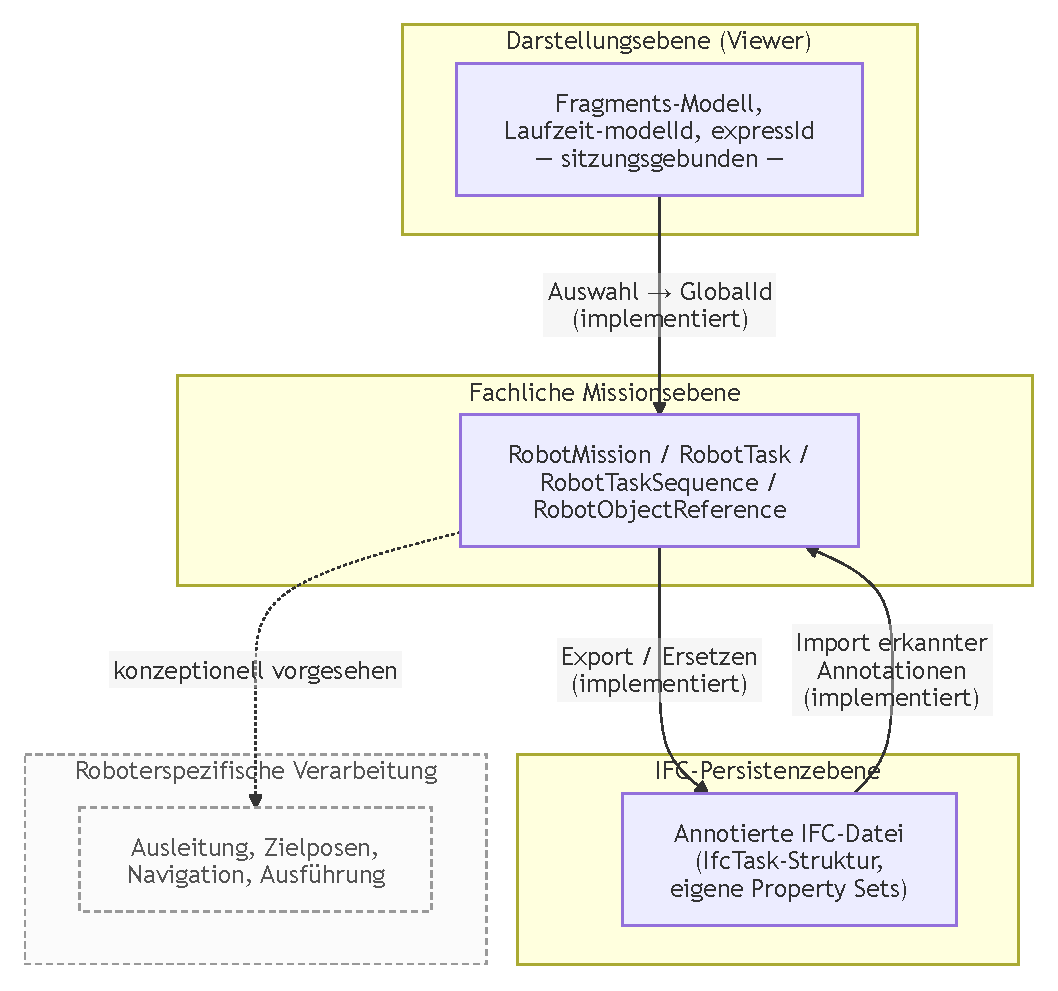
\includegraphics[width=0.4\textwidth]{pics/abbildung_4-1_trennung_der_ebenen.pdf}
    \caption{Trennung der Ebenen}
    \label{fig:trennung-der-ebenen}
\end{figure}

Zu unterscheiden sind das fachliche Missions- und Aufgabenmodell, die IFC-Repräsentation dieses
Modells und die Darstellungsstruktur des Viewers. Das fachliche Modell ist als eigenständige Schicht
konzipiert, die weder von Kennungen der Darstellungsstruktur noch von einer Persistenztechnologie
oder der konkreten STEP-Syntax abhängt. Zwischen Domäne und IFC liegt eine gesonderte
Abbildungsebene, sodass die fachlichen Mappingregeln unabhängig von Dateizugriff und Viewerzustand
prüfbar bleiben. Das daraus abgeleitete Modellierungsziel lautet, dass Robotermissionsdaten nicht
von temporären Rendering-Strukturen oder viewer-spezifischen Kennungen abhängig sein dürfen. Die
technische Ausgestaltung dieser Schichtung ist Gegenstand von Kapitel~\ref{sec:Editor}. Für die
Modellkonzeption ist maßgeblich, dass die fachliche Aussage einer Annotation unabhängig von der Art
ihrer Darstellung und Serialisierung gültig bleibt.

Das fünfte Ziel betrifft IFC als Träger der Annotation in beide Richtungen. Missionsinformationen
sollen so weit sinnvoll in der IFC-Struktur selbst abgebildet werden, dass Gebäudeinformation und
Missionsbezug gemeinsam transportiert werden können und keine zweite, separat zu pflegende
Hauptdatenquelle entsteht. Im untersuchten System ist dazu nicht nur der Export einer Mission in die zugrunde
liegende IFC-Quelldatei umgesetzt, sondern auch das umgekehrte Wiedereinlesen: Vom System selbst
erzeugte, projekteigene Missionsannotationen werden beim Laden einer IFC-Datei erkannt und zu
RobotMission- und RobotTask-Aggregaten rekonstruiert. Eine importierte Mission kann im Editor
verändert und anschließend erneut exportiert werden, wobei der zuvor erkannte Missionsgraph gezielt
ersetzt statt bei jedem Durchlauf neu angehängt wird. Nach dem Export wird die erzeugte Datei zur
Absicherung erneut geöffnet, die Mission erneut importiert und mit dem beabsichtigten Domänenmodell
semantisch verglichen, bevor die neuen Bytes als Ausgangspunkt für den nächsten Zyklus übernommen
werden. Für deterministisch wiedererkennbare Missionsentitäten bleiben bestehende IFC-GlobalIds über
solche Zyklen hinweg erhalten. Bestehende Building-GlobalIds werden dabei nicht angetastet. Dennoch
ist eine Abgrenzung notwendig: Der implementierte Roundtrip bezieht sich ausschließlich auf den vom
System erkannten, projekteigenen Missionsgraphen. Strukturelle Änderungen am Gebäudemodell selbst
werden nicht zurückgeschrieben, Modelle ohne erhaltene IFC-Quelle sind nicht exportierbar, und nicht
jedes IFC-Schema wird vom Missionswriter unterstützt. Ein verlustfreier Roundtrip beliebiger
Modelländerungen ist damit ausdrücklich nicht Gegenstand dieses Roundtrips.

Aus dem Anspruch, das Modell langfristig erweiterbar zu halten, folgt als sechstes Ziel
die Erweiterbarkeit. Zusätzliche Aktionsarten, weitere Aufgabeneigenschaften, differenziertere
Objektrollen, weitere zeitliche Beziehungsarten und roboterspezifische Ausleitungen sollen ergänzt
werden können, ohne die Grundstruktur neu entwerfen zu müssen. Die Aktionssemantik liegt hierzu in
einem klar abgegrenzten, überwiegend optional besetzten Eigenschaftsbereich der Aufgabe.
Objektrollen werden über benannte Relationen und nicht über strukturell verschiedene Modellelemente
unterschieden. Eine explizite Schemaversion wird in jede exportierte Mission geschrieben, sodass
ältere Annotationsstände beim Einlesen erkennbar und behandelbar bleiben.

Als siebtes Ziel ist die Validierbarkeit zu nennen. Eine Annotation, die sowohl exportiert als auch
wieder importiert werden soll, muss vor der Weitergabe überprüfbar sein. Das Validierungsmodell unterscheidet
dabei durchgängig zwischen blockierenden Fehlern und nicht blockierenden Warnungen: Unvollständige
Entwürfe bleiben bearbeitbar, während sowohl die Abbildung in IFC-nahe Records als auch der
tatsächliche Export nur für Missionen zugelassen werden, die vollständig gültig sind und deren
Objektbezüge im gewählten Quellmodell eindeutig aufgelöst werden können. Fehlende Typinformationen
des referenzierten Bauteils führen zu einer Warnung statt zu einer Zurückweisung einer ansonsten
plausiblen Aufgabe. Ein bekannter, aber unpassender Objekttyp führt dagegen zu einem blockierenden
Fehler.

Die Frage der Interoperabilität ist demgegenüber differenziert zu beantworten. Das Modell verwendet
für Struktur und Beziehungen reguläre IFC-Entitäten, sodass eine annotierte Datei syntaktisch gültig
bleibt und die Missionsstruktur von generischen Werkzeugen als Prozessstruktur gelesen werden kann.
Die eigentliche Robotiksemantik, also die Aktionswerte und die Bedeutung der eigenen Eigenschaftsgruppen,
 ist hingegen projektspezifisch und nicht Bestandteil des IFC-Standards. Daraus folgt, dass die
strukturelle Lesbarkeit durch Fremdsysteme angenommen werden kann, die inhaltliche Interpretation
der Robotiksemantik durch Fremdsysteme jedoch nicht. Ein Nachweis der tatsächlichen Interpretation
durch andere Werkzeuge wurde im Rahmen dieser Arbeit nicht geführt.

Schließlich soll das Annotationsmodell die fachliche Grundlage für eine spätere Verarbeitungskette
bilden, die von der IFC-Annotation über das interne Missionsmodell zu einer roboterspezifischen
Ausleitung, zu Zielposen und Navigationsdaten und letztlich zur Ausführung führt. Von dieser Kette
ist im vorliegenden Stand der vordere, bidirektionale Teil (Export, Import und verifizierter
Roundtrip) umgesetzt. Die roboterspezifische Weiterverarbeitung ist konzeptionell vorgesehen und
wird in Kapitel~\ref{sec:Weiterführung} behandelt. Für die Modellierung ist diese Abgrenzung dennoch bedeutsam, weil sie
begründet, weshalb Aktionsart, Objektbezug, Objektrolle und Reihenfolge explizit und getrennt
voneinander repräsentiert werden müssen: Erst diese Explizitheit erlaubt es, aus einer Annotation
später eine ausführbare Anweisung abzuleiten, ohne fachliche Annahmen aus einer Darstellungsform
rekonstruieren zu müssen. Abbildung~\ref{fig:grundstruktur_annotationsmodell} fasst die daraus resultierende Grundstruktur zusammen.
\begin{figure}[htbp]
    \centering
    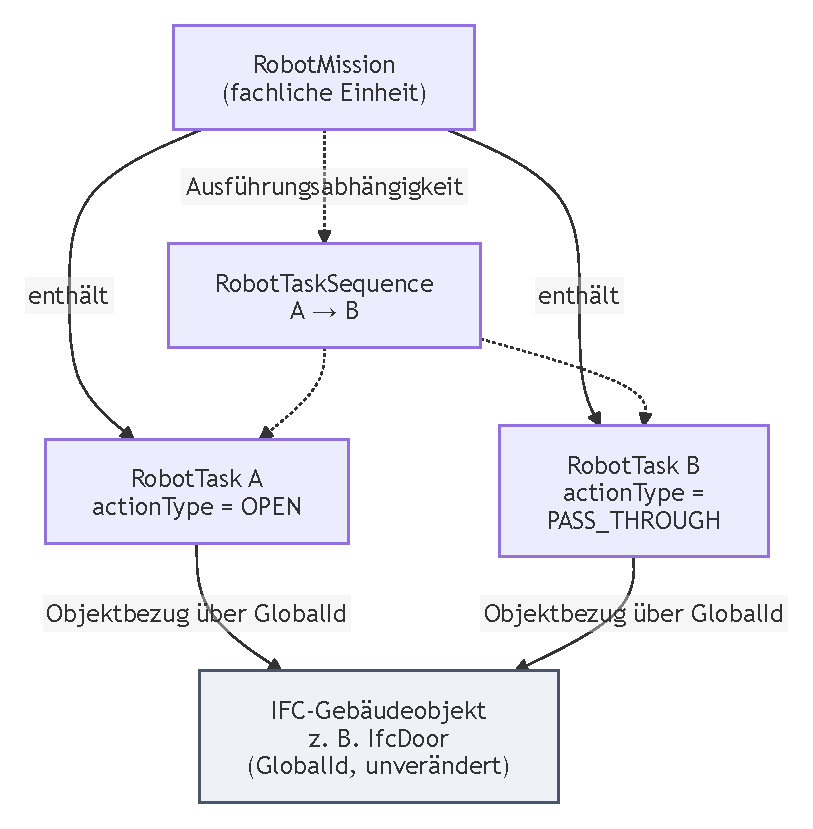
\includegraphics[width=0.4\textwidth]{pics/abbildung_4-2_grundstruktur_annotationsmodell.pdf}
    \caption{Grundstruktur Annotationsmodell}
    \label{fig:grundstruktur_annotationsmodell}
\end{figure}


Die in diesem Abschnitt formulierten Ziele bleiben zunächst Anforderungen an das Datenmodell. Wie
sie durch ein konkretes internes Domänenmodell mit Missionen, Aufgaben, Sequenzen, Objektbezügen und
Aktionsparametern eingelöst werden, ist Gegenstand des folgenden Abschnitts.

\subsection{Internes Domänenmodell}\label{subsec:Internes_Domänenmodell}
Aus den zuvor formulierten Modellierungszielen wird im Folgenden das interne Domänenmodell
abgeleitet. Während Abschnitt~\ref{subsec:modellierungsziele-annotationsmodell} begründet hat, welche
fachlichen Sachverhalte repräsentiert werden müssen, beschreibt dieses Unterkapitel die
Verantwortlichkeiten und Beziehungen der dafür vorgesehenen Domänenkonzepte. Leitend ist die Frage,
wie Robotermissionen unabhängig von IFC-Serialisierung, Viewer und Benutzeroberfläche fachlich
repräsentiert werden können.

Das Domänenmodell bildet die fachliche Zwischenschicht des Systems. Es umfasst die Beschreibung von
Missionen, Tasks, Sequenzen, Objektbezügen und Zeitinformationen sowie die zugehörigen Erzeugungs-,
Änderungs- und Validierungsregeln. Weder die dreidimensionale Darstellung eines Gebäudemodells noch
die konkrete IFC-Syntax bestimmen, wie eine Mission fachlich beschrieben wird. Das Domänenmodell
ist damit nicht lediglich ein technisches Zwischenformat, sondern die maßgebliche fachliche
Repräsentation, aus der sowohl der Editorzustand als auch die IFC-Repräsentation abgeleitet und in
die beide wieder zurückgeführt werden können.
Abbildung~\ref{fig:grundstruktur_domaenenmodell} zeigt die Struktur des Modells im Überblick.

\begin{figure}[htbp]
    \centering
    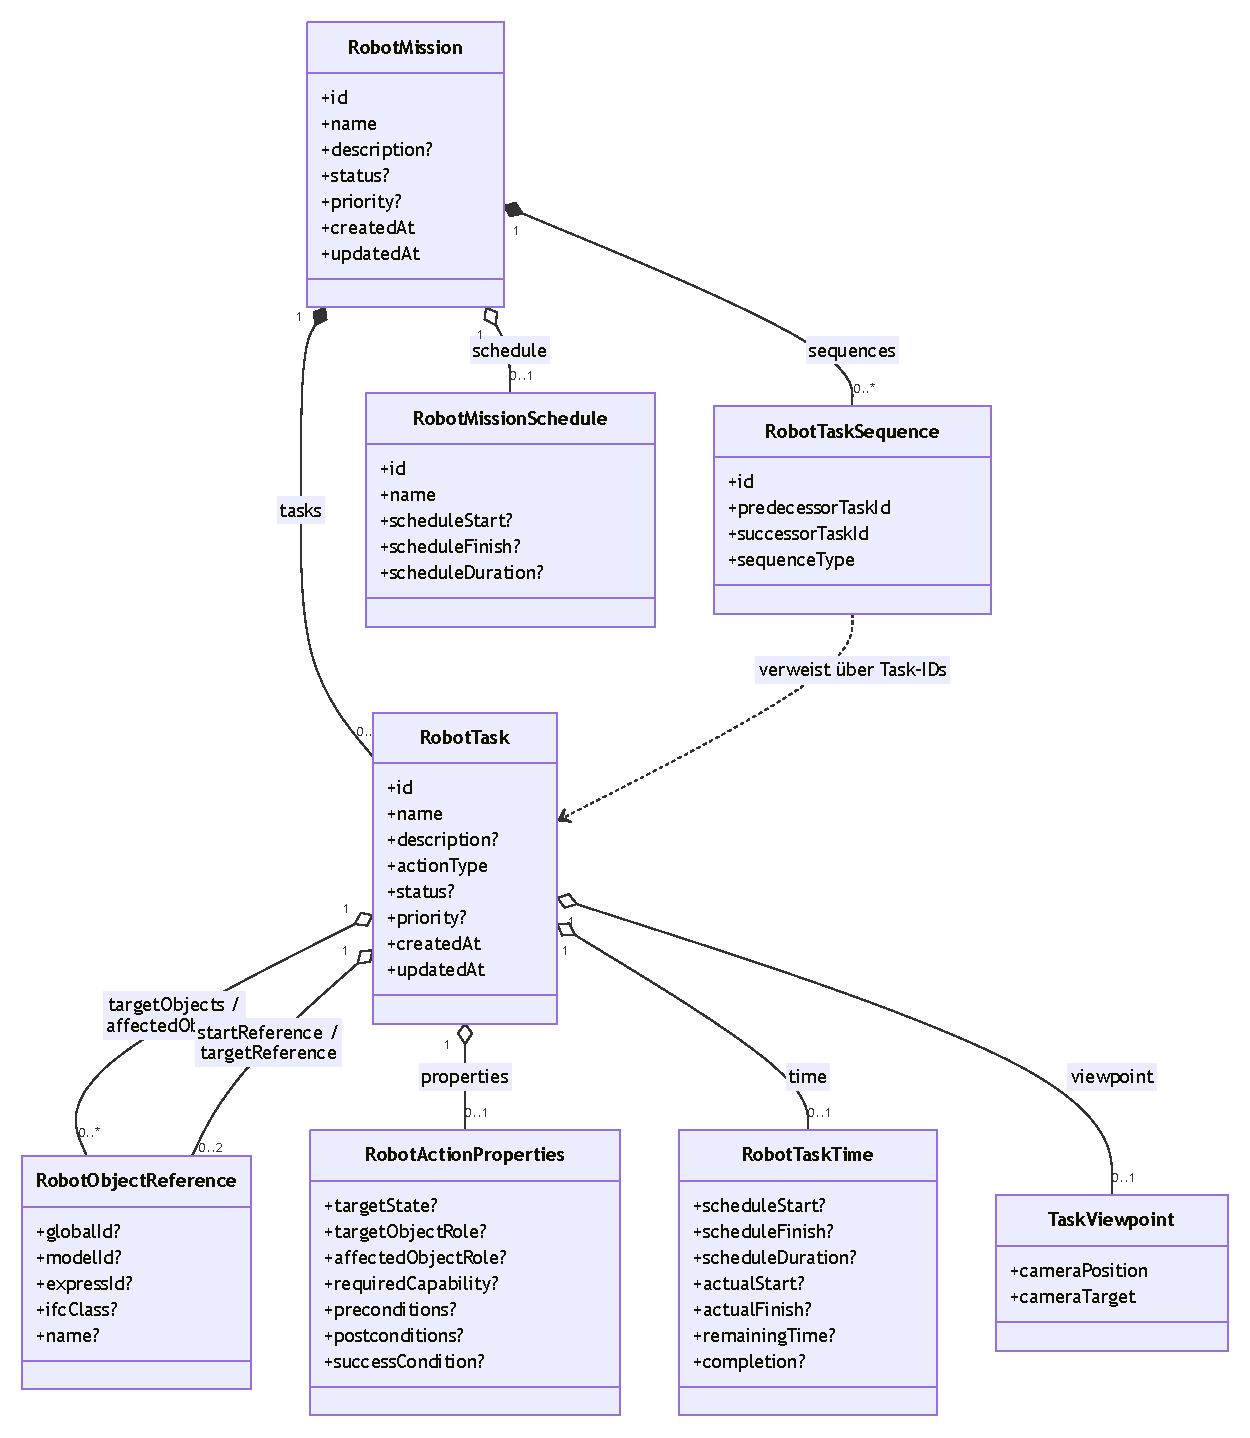
\includegraphics[width=0.7\textwidth]{pics/struktur_internes_domänenmodell.pdf}
    \caption{Struktur des internen Domänenmodells}
    \label{fig:grundstruktur_domaenenmodell}
\end{figure}
\subsubsection{Die Mission als übergeordnete Einheit}\label{Mission_Einheit}
\textit{RobotMission} bezeichnet eine vollständige Robotermission und bildet die übergeordnete Einheit des
Modells, also diejenige Struktur, über die alle zugehörigen Informationen erreichbar sind und deren
Konsistenz als Ganzes geprüft werden kann. Sie bildet damit das fachliche Aggregat der
Missionsbeschreibung. Entscheidend ist, dass ausführbare Schritte, deren
Abhängigkeiten und die optionale Zeitplanung nicht unabhängig voneinander existieren, sondern stets
im Kontext genau einer Mission.

Eine Mission trägt eine stabile anwendungsseitige Kennung (\textit{id}), einen menschenlesbaren Namen sowie
eine optionale Beschreibung. Die Kennung ist ausdrücklich eine Anwendungs-ID und keine
IFC-Identität. Die Frage, wie beide Identitätsräume beim Export und Import aufeinander abgebildet
werden, wird in Abschnitt~\ref{subsec:modell_ifc} und hinsichtlich der technischen Verarbeitung in
Kapitel~\ref{sec:Editor} behandelt. Ergänzend führt die Mission einen
aggregierenden Bearbeitungsstatus und eine Priorität. Bemerkenswert ist, dass Status und Priorität
im Modell durch dieselben Typen beschrieben werden wie auf Task-Ebene. Mission und Task teilen damit
dasselbe Vokabular für Lebenszyklus und Dringlichkeit, was den Aufbau der Bearbeitungsoberfläche
vereinheitlicht.

Die eigentliche fachliche Substanz liegt in drei Feldern. \textit{tasks} enthält die ausführbaren
Einzelschritte der Mission, \textit{sequences} die expliziten gerichteten Abhängigkeiten zwischen diesen
Schritten, und \textit{schedule} optional eine Zeitplanung der Mission als Ganzes. Hinzu kommen ein
Erstellungs- und ein Änderungszeitstempel, die nachvollziehbar machen, wann eine Mission zuletzt
bearbeitet wurde. Wesentlich ist, dass die Mission selbst keine Roboteraktion beschreibt: Sie ist
Container und Klammer, nicht ausführbare Handlung. Jede konkrete Tätigkeit wird ausschließlich durch
die enthaltenen Tasks ausgedrückt.

\subsubsection{Der Task als ausführbare Einheit}\label{Task_Einheit}
\textit{RobotTask} bezeichnet einen ausführbaren Einzelschritt innerhalb einer Mission. Der Task ist die
zentrale Struktur des Modells, weil er unterschiedliche Informationsbereiche zusammenführt, die im
Modell dennoch klar getrennt bleiben.

Den fachlichen Kern bildet die Aktion: Jeder Task besitzt neben Kennung, Name und optionaler
Beschreibung genau einen \textit{actionType}, also die konkrete auszuführende Roboteraktion. Der zweite
Bereich umfasst die Bezüge zu Gebäudeelementen. Hier unterscheidet das Modell zwischen
\textit{targetObjects} als unmittelbar adressierten oder als Kontext genutzten Objekten und
\textit{affectedObjects} als indirekt betroffenen Objekten. Für Bewegungsaufgaben treten zusätzlich
\textit{startReference} und \textit{targetReference} als Ausgangs- und Zielbezug hinzu. Der dritte Bereich sind
die Aktionsparameter (\textit{properties}), der vierte die zeitlichen Informationen (\textit{time}). Als fünfter,
optionaler Bereich können mit \textit{viewpoint} und \textit{markerPosition} annotationsbezogene
Zusatzinformationen hinterlegt werden, die den Task im Viewer wiederauffindbar machen. Abgeschlossen
wird die Struktur durch Status, Priorität und Zeitstempel.

Abstrahiert ergibt sich damit folgender Aufbau:
\begin{figure}[htbp]
    \centering
    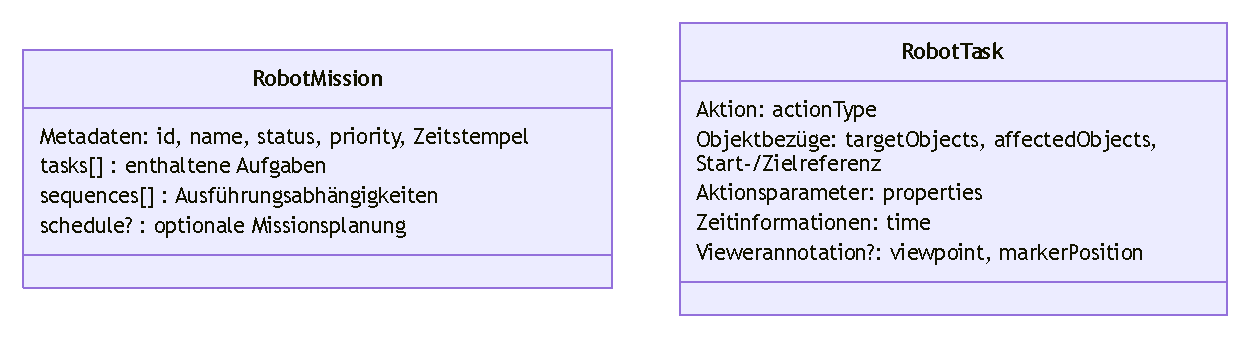
\includegraphics[width=0.4\textwidth]{pics/Attributstruktur.pdf}
    \caption{Attributstruktur RobotMission und RobotTask}
    \label{fig:Attributstruktur}
\end{figure}

Die Trennung dieser Bereiche ist keine bloße Ordnungsfrage. Sie erlaubt es, denselben Task
schrittweise anzureichern. Zunächst Aktion und Zielobjekt, später Parameter und Zeitplanung, ohne
dass unvollständige Zwischenstände strukturell unzulässig wären. Zugleich stellt sie sicher, dass
die einzelnen Bereiche später auf unterschiedliche IFC-Konstrukte abgebildet werden können, ohne im
Domänenmodell vermischt zu sein.

\subsubsection{Referenzen und ergänzende Wertobjekte}\label{Ref_Ojekte}
\textit{RobotObjectReference} bezeichnet den fachlichen Verweis auf ein IFC-Objekt. Entscheidend ist, dass
im Domänenmodell keine Viewer- oder Three.js-Objekte, keine Geometrie und keine Rendering-Handles
gespeichert werden, sondern ausschließlich eine schlanke Identitätsbeschreibung. Bevorzugt wird die
\textit{globalId}, also die dauerhafte IFC-Objektidentität. Steht diese nicht zur Verfügung, ist ein
modelllokaler Fallback aus \textit{modelId} und \textit{expressId} zulässig. Die Typdefinition erzwingt dabei
bereits auf Typebene, dass eine \textit{expressId} ohne \textit{globalId} nur zusammen mit der zugehörigen
\textit{modelId} verwendet werden kann, da Express-IDs nur innerhalb einer Modellserialisierung eindeutig
sind. Ergänzend können mit \textit{ifcClass} und \textit{name} beschreibende Angaben zum Objekt geführt werden.
Die vollständige Referenzierungsstrategie einschließlich ihrer Konsequenzen für Modellgrenzen und
wiederholte Serialisierungen ist Gegenstand von
Abschnitt~\ref{subsec:Referenzierung_IFC-Objekten}.

Wesentlich für das Verständnis des Modells ist, dass die Referenz bewusst frei von Aktionssemantik
bleibt. Sie beantwortet die Frage, welches Bauteil gemeint ist, nicht die Frage, was mit ihm
geschehen soll. Diese zweite Frage beantwortet \textit{RobotActionProperties}, also die strukturierte
Beschreibung der konkreten Aktionsanforderung eines Tasks. Dort können unter anderem ein
angestrebter Zielzustand, die semantischen Rollen der adressierten und der betroffenen Objekte, eine
erforderliche Roboterfähigkeit sowie Vor-, Nachbedingungen und ein Erfolgskriterium hinterlegt
werden. Da diese Angaben am Task und nicht am Objekt hängen, kann dasselbe IFC-Objekt in
verschiedenen Tasks mit unterschiedlichen Anforderungen verwendet werden. Etwa eine Tür, die in
einem Schritt geöffnet und in einem späteren wieder geschlossen wird. Die Bedeutung der einzelnen
Aktionsarten wird in Abschnitt~\ref{subsec:Modellierung_Roboteraktionen} behandelt.

\textit{RobotTaskTime} bezeichnet die zeitliche Beschreibung eines einzelnen Tasks und umfasst geplanten
Start, geplantes Ende und geplante Dauer, den tatsächlichen Start und das tatsächliche Ende, die
verbleibende Dauer sowie einen Fertigstellungsgrad. Diese Angaben sind bewusst nicht Teil von
\textit{RobotActionProperties}, obwohl beide Strukturen den Task ergänzen. Aktionsparameter beschreiben die
fachliche Anforderung an die Ausführung und sind projektspezifisch. Zeitangaben beschreiben dagegen
Planung und Fortschritt und entsprechen einem in IFC bereits vorhandenen Konzept, das in
Abschnitt~\ref{subsec:Taskinformationen} aufgegriffen wird. Die Trennung im Domänenmodell nimmt diese unterschiedliche Herkunft vorweg und
vermeidet, dass Planungsdaten in einer projekteigenen Parameterstruktur verborgen werden.

Auf Missionsebene existiert mit \textit{RobotMissionSchedule} eine optionale Zeitplanung für die Mission
als Ganzes, bestehend aus Kennung, Name sowie geplantem Start, Ende und Dauer. Sie ersetzt die
Task-Zeiten nicht, sondern beschreibt einen übergeordneten Rahmen: Der Task-Zeitbereich betrifft die
Ausführung eines einzelnen Schritts einschließlich des tatsächlichen Verlaufs, die Missionsplanung
dagegen ausschließlich die geplante zeitliche Einordnung des Gesamtvorgangs.

\subsubsection{Hierarchie und Ausführungsabhängigkeit als getrennte Strukturen}
\textit{RobotTaskSequence} bezeichnet eine eigenständige gerichtete Abhängigkeit zwischen zwei Tasks. Eine
Sequenz besitzt eine eigene stabile Kennung, verweist über Task-IDs auf einen Vorgänger und einen
Nachfolger und trägt einen Sequenztyp, der die Art der zeitlichen Beziehung angibt. Sequenzen sind
damit eigenständige Elemente der Mission und keine Eigenschaft eines Tasks.

Daraus ergibt sich die für dieses Kapitel zentrale Unterscheidung: \textit{RobotMission.tasks} beschreibt,
welche ausführbaren Schritte zur Mission gehören, und legt zugleich deren deterministische
Darstellungs- und Hierarchieordnung fest. \textit{RobotMission.sequences} beschreibt demgegenüber, welche
zeitlichen Abhängigkeiten zwischen diesen Schritten bestehen. Beide Strukturen ließen sich nicht
ohne Informationsverlust durch ein einziges sortiertes Task-Array ersetzen. Ein Array kann
ausschließlich eine lineare Folge ausdrücken. Ein Abhängigkeitsgraph kann darüber hinaus unabhängige
Zweige und mehrere Vorgänger desselben Nachfolgers darstellen. Zwei Tasks, die in beliebiger
Reihenfolge oder parallel ausgeführt werden dürfen, sind in einem Array zwangsläufig geordnet, im
Graphen dagegen korrekt als unabhängig beschreibbar.
Abbildung~\ref{fig:Missionsstruktur_ausführung} stellt beide Sichten einander gegenüber.
\begin{figure}[htbp]
    \centering
    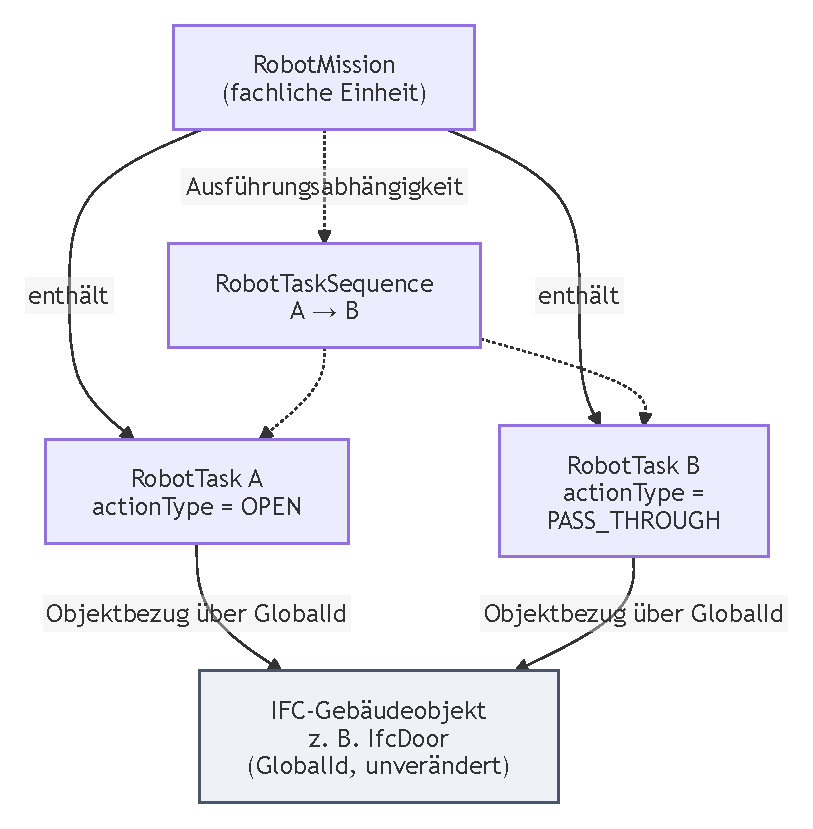
\includegraphics[width=0.7\textwidth]{pics/Missionsstruktur.pdf}
    \caption{Gegenüberstellung der Missionsstruktur und der Ausführungsabhängigkeiten}
    \label{fig:Missionsstruktur_ausführung}
\end{figure}

Die Implementierung behandelt beide Strukturen konsequent getrennt. Die Sequenzlogik prüft den
Graphen auf Selbstbezüge, auf Verweise auf unbekannte Tasks und auf Zyklen und kann aus Hierarchie
und Sequenzen eine ausführungsgerechte Reihenfolge ableiten, wobei die Hierarchieordnung als
deterministisches Tie-Breaking-Kriterium für voneinander unabhängige Tasks dient. Legt eine
Anwenderin oder ein Anwender eine rein lineare Reihenfolge fest, wird daraus eine vollständige Kette
vom Typ \textit{FINISH\_START} erzeugt. Auch dieser Fall wird jedoch als Sequenzgraph gespeichert und nicht
auf die Array-Reihenfolge reduziert. Die inhaltliche Semantik der Sequenztypen sowie die
Zyklusbehandlung im Detail sind Gegenstand von Abschnitt~\ref{subsec:Hierarchie_sequenzen}.

\subsubsection{Domänenoperationen und Invarianten}
Damit das Modell nicht nur beschreibend, sondern auch verlässlich ist, werden Änderungen durch
definierte Domänenoperationen ausgedrückt. Diese umfassen insbesondere das Hinzufügen von Tasks, die
Zuweisung von Ziel- und betroffenen Objekten, das Setzen von Start- und Zielbezügen einer
Bewegungsaufgabe sowie Änderungen an Aktionsparametern und Zeitangaben.

Vier Eigenschaften dieser Operationen prägen das Modell. Erstens werden Eingaben normalisiert:
Pflichttexte wie Kennungen und Namen werden bereinigt, und eine leere Angabe führt unmittelbar zu
einem Domänenfehler statt zu einem strukturell gültigen, fachlich aber unbrauchbaren Objekt.
Zweitens erzeugt jede Änderung eine neue Objektstruktur, statt bestehende Objekte zu verändern.
Missionen und Tasks werden also als unveränderliche Werte behandelt, was Vergleiche zwischen einem
beabsichtigten und einem rekonstruierten Zustand erst zuverlässig möglich macht. Drittens werden
Eindeutigkeitsregeln früh durchgesetzt: Task-Kennungen müssen innerhalb einer Mission eindeutig
sein, weil Sequenzen genau über diese Kennungen auflösen, und dieselbe Objektidentität wird einem
Task nicht mehrfach zugewiesen. Viertens wird bei jeder Änderung der Änderungszeitpunkt
fortgeschrieben.

Ergänzend prüft eine eigene Validierung die fachlichen Invarianten des Modells und meldet
blockierende Fehler und nicht blockierende Warnungen als maschinen- und menschenlesbare Befunde. Für
dieses Kapitel ist vor allem bemerkenswert, dass die Validierung die Trennung von Objekt und Aktion
ausdrücklich absichert: Aktionsparameter, die an einer Objektreferenz statt am Task hinterlegt
wurden, werden als Verstoß gemeldet. Die vollständigen
Regeln werden in Abschnitt~\ref{subsec:validierungsmodell} dargestellt.

\subsubsection{Frameworkunabhängigkeit und gemeinsame Repräsentation im Roundtrip}
Die Domänenschicht ist frei von direkten Abhängigkeiten zu Darstellungsbibliotheken, Viewerzustand,
IFC-Verarbeitung und Browser-Persistenz. Äußere Systembereiche verwenden die Domänenkonzepte, ohne
ihre technischen Strukturen in die Domäne einzubringen. Eine Auswahl im dreidimensionalen Modell
wird beispielsweise vor der Übergabe an die Domäne in eine \textit{RobotObjectReference}
übersetzt. Die Domäne kennt anschließend nur diese fachliche Referenz und nicht mehr das
Auswahlobjekt, aus dem sie entstanden ist. Damit wird die Frage, wie eine Mission beschrieben wird,
unabhängig davon beantwortet, wie sie dargestellt, gespeichert oder serialisiert wird:

\begin{figure}[htbp]
    \centering
    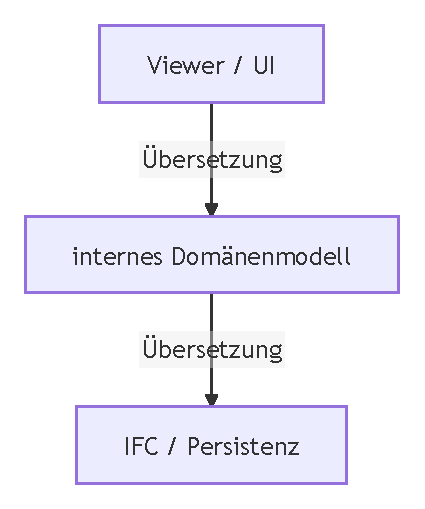
\includegraphics[width=0.4\textwidth]{pics/Schichten_pipeline.pdf}
    \caption{Pipeline}
    \label{fig:Pipeline}
\end{figure}

Die technische Umsetzung dieser Schichtung ist Gegenstand von Kapitel~\ref{sec:Editor}. Für das Datenmodell
selbst ist entscheidend, dass Auswahlmechanismen, Renderingstrukturen und Dateiformate keinen
Eingang in die fachliche Beschreibung finden.

Diese Unabhängigkeit ist zugleich die Voraussetzung dafür, dass das Modell im implementierten
IFC-Roundtrip als gemeinsamer Bezugspunkt dienen kann. Erstellte Missionen, aus einer
annotierten IFC-Datei rekonstruierte Missionen, im Editor bearbeitete Missionen und erneut zu
exportierende Missionen werden durch dieselben Typen beschrieben. Beide Richtungen des Austauschs
greifen dabei nicht nur auf dieselben Typen, sondern auch auf dieselbe Domänenvalidierung zurück:
Sowohl die Rekonstruktion einer Mission aus IFC als auch die Abbildung einer Mission auf IFC-nahe
Strukturen prüfen das Ergebnis gegen die fachlichen Invarianten des Domänenmodells. Konzeptionell
gilt damit: IFC-Import und IFC-Export treffen sich im selben internen Domänenmodell. Dass
dieselbe Struktur beide Richtungen bedient, ist auch der Grund dafür, dass Hierarchie und Sequenzen
getrennt geführt werden – nur so bleiben beide Informationen beim Rücklesen unterscheidbar. Die
Implementierung von Import, Replacement-Export und semantischem Vergleich wird in
Kapitel~\ref{sec:Editor} behandelt.

\subsection{Modellierung der Roboteraktionen}\label{subsec:Modellierung_Roboteraktionen}
\subsubsection{Aktionsart als Pflichtangabe des Tasks}
Jeder ausführbare Schritt einer Mission wird durch einen \textit{RobotTask} repräsentiert, der die
beabsichtigte Roboteraktion als Pflichtangabe trägt. Für den betrachteten Anwendungsfall umfasst der
zulässige Wertebereich \textit{OPEN}, \textit{CLOSE}, \textit{SWITCH\_ON}, \textit{SWITCH\_OFF},
\textit{MOVE}, \textit{PASS\_THROUGH} und \textit{NAVIGATE\_TO}. Unbekannte oder fehlende Werte
werden als eigene Validierungsbefunde behandelt, sodass auch aus persistenten Daten rekonstruierte
Missionen gegen dasselbe Vokabular geprüft werden. Die Aktionswerte sind projektspezifische
Bezeichner und keine native IFC-Enumeration. Der Modellierungsbeitrag liegt dabei nicht in der
Erfindung semantischer Roboteraktionen, sondern in ihrer expliziten Trennung vom referenzierten
Gebäudeobjekt und ihrer Einbettung in die rekonstruierbare Mission.
\subsubsection{Abstraktionsgrad der Aktionsbezeichner}
Die verwendeten Aktionsarten sind als semantische Bezeichner auf fachlicher Ebene zu verstehen.
Sie benennen den fachlich beabsichtigten Zielzustand oder Vorgang, nicht den technischen Ablauf auf
Roboterebene. Der Bezeichner OPEN beschreibt, dass ein Bedienobjekt anschließend als geöffnet gelten
soll. Er legt weder eine Anfahrstrategie noch eine Greif- oder Betätigungsstrategie fest. Auf
Robotikseite kann derselbe Task auf eine deutlich längere Handlungskette abgebildet werden, etwa:
Objekt anfahren, Bedienelement erkennen, Manipulationspose bestimmen, Betätigung ausführen und das
Ergebnis überprüfen. Der IFC-basierte Task beschreibt somit primär, was erreicht werden soll,
während die spätere roboterspezifische Ausführung festlegt, wie dieses Ziel erreicht wird. Diese
Zurückhaltung ist eine Modellierungsentscheidung: Eine Annotation, die bereits Bewegungsprimitive
oder Skill-Parameter enthielte, wäre an eine konkrete Roboterplattform gebunden und im Gebäudemodell
nicht mehr allgemein interpretierbar.

\begin{figure}[htbp]
    \centering
    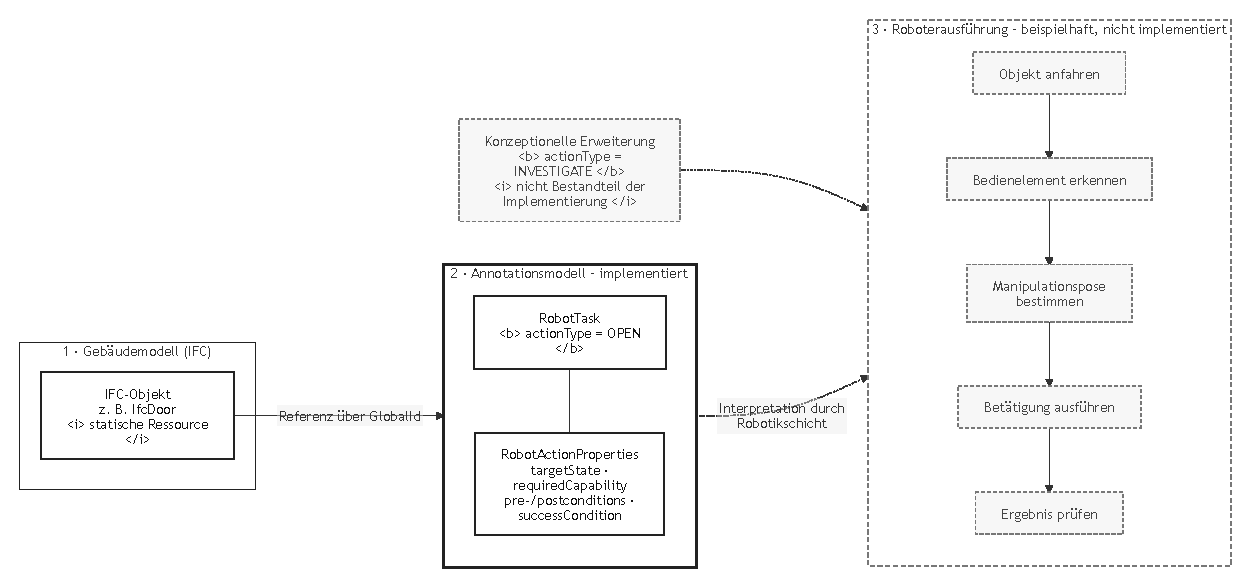
\includegraphics[width=0.8\textwidth]{pics/Abstraktionsebenen_Aktionsmodellierung.pdf}
    \caption{Abstraktionsebenen der Aktionsmodellierung.}
    \label{fig:Abstraktionsebenen-Aktionsmodellierung}
\end{figure}

Abbildung~\ref{fig:Abstraktionsebenen-Aktionsmodellierung} stellt der semantischen Beschreibung am
\textit{RobotTask} beispielhafte roboterspezifische Ausführungsketten gegenüber. Die dort ebenfalls
gezeigte Aktion \textit{INVESTIGATE} kennzeichnet ausschließlich eine mögliche Erweiterung.


\subsubsection{Erweiterbarkeit der Aktionssemantik}
Der vorliegende Wertebereich ist kein abschließender Aktionskatalog, sondern der Umfang des
betrachteten Anwendungsfalls. Eine Ergänzung des Vokabulars muss konsistent in Domänenmodell,
Validierung, IFC-Abbildung und Editor nachvollzogen werden. Als konzeptionelles Beispiel
lässt sich eine Aktion INVESTIGATE denken, die einen definierten Bereich untersuchen, dort
hinterlegte Handlungsanweisungen erfassen, eine Informationsquelle wie einen QR-Code erkennen, deren
Inhalt interpretieren und daraus weitere roboterspezifische Aktionen ableiten würde. Weder
INVESTIGATE noch eine QR-Code-Verarbeitung sind Bestandteil der aktuellen Implementierung. Das
Beispiel dient ausschließlich dazu, die angestrebte Abstraktionsebene zu verdeutlichen. Es zeigt
zugleich, dass auch eine im Ablauf sehr komplexe Aktion auf Modellebene ein einzelner semantischer
Bezeichner bleiben kann, sofern die Interpretation der Ausführungsschicht überlassen wird.

\subsubsection{Ergänzende Aktionssemantik über \textit{RobotActionProperties}}
Der \textit{actionType} allein ist häufig zu grob, um eine Aufgabe eindeutig zu beschreiben. \textit{RobotTask}
besitzt deshalb das optionale Feld \textit{properties} vom Typ \textit{RobotActionProperties}, dessen sämtliche
Felder ihrerseits optional sind: \textit{targetState} benennt den erwarteten Zustand nach der Ausführung,
\textit{targetObjectRole} und \textit{affectedObjectRole} präzisieren die semantische Rolle der referenzierten
Objekte, \textit{requiredCapability} benennt die erforderliche Roboterfähigkeit, \textit{preconditions} und
\textit{postconditions} halten Bedingungen vor und nach der Ausführung fest, und \textit{successCondition}
beschreibt das beobachtbare Erfolgskriterium. Ein Task mit \textit{actionType = OPEN} kann damit um einen
gewünschten Zielzustand, eine benötigte Fähigkeit, Vor- und Nachbedingungen sowie ein
Erfolgskriterium ergänzt werden, ohne dass die Aktionsart selbst weiter ausdifferenziert werden
muss. Die Werte sind als Freitext modelliert; kontrollierte Vokabulare sind im betrachteten Modell
nicht vorgegeben.
\subsubsection{Trennung von Aktion und IFC-Objekt}
Die konkrete Aktionssemantik gehört ausschließlich zum \textit{RobotTask} und nicht zur Objektreferenz.
\textit{RobotObjectReference} trägt nur Identitäts- und Beschreibungsdaten wie \textit{globalId}, \textit{modelId},
\textit{expressId}, \textit{ifcClass} und \textit{name}; eine angeforderte Roboteraktion gehört nicht
zu dieser Referenz. Diese Regel wird strukturell ausgedrückt und bei rekonstruierten Daten validiert.
Fachlich bedeutet das, dass eine \textit{IfcDoor} ein Gebäudeelement bleibt und keine
Missionsabsicht trägt. Mehrere Tasks können dieselbe Tür in der Folge \textit{NAVIGATE\_TO},
\textit{OPEN}, \textit{PASS\_THROUGH} und \textit{CLOSE} referenzieren, ohne den persistenten
Gebäudebezug zu verändern.
Ebenso können mehrere Missionen unabhängig voneinander auf dasselbe Gebäudemodell verweisen. Die
Aktionsart wirkt lediglich als Interpretationsrahmen für die Referenzen: Für \textit{MOVE} sind Start- und
Zielreferenz erforderlich, \textit{PASS\_THROUGH} verlangt mindestens eine Referenz, und bei \textit{OPEN},
\textit{CLOSE}, \textit{SWITCH\_ON} und \textit{SWITCH\_OFF} wird die bekannte IFC-Klasse auf Plausibilität geprüft,
während fehlende Klasseninformation nur zu einer Warnung führt. Diese Kopplung bleibt damit bewusst
schwach. Die Prüflogik selbst wird in Abschnitt~\ref{subsec:validierungsmodell} behandelt.
\subsubsection{Einordnung zwischen Gebäudemodell und Roboterausführung}
Aus den beschriebenen Entscheidungen ergibt sich eine dreistufige Abstraktion: Das Gebäudeobjekt
beschreibt die statische Ressource, der semantische \textit{RobotTask} beschreibt die beabsichtigte Wirkung
auf diese Ressource, und die roboterspezifische Ausführung beschreibt die tatsächliche
Handlungskette. Der Editor deckt gegenwärtig ausschließlich die mittlere Ebene ab. Aspekte wie
Manipulationsplanung, Bildverarbeitung, Waypoint-Erzeugung oder konkrete Roboter-Skills sind nicht
Gegenstand des Annotationsmodells und werden hier nur als mögliche Interpretationen einer abstrakten
Aktion erwähnt. Damit bleibt das Modell gegenüber unterschiedlichen Roboterplattformen offen, und
die Verantwortung für die Ausführbarkeit verbleibt in der nachgelagerten Robotikschicht.

\subsection{Referenzierung von IFC-Objekten}\label{subsec:Referenzierung_IFC-Objekten}
Ein \textit{RobotTask} beschreibt eine Handlung, die sich auf ein konkretes Bauteil des
Gebäudemodells bezieht. Etwa eine Tür, die geöffnet, oder einen Raum, der durchquert werden soll.
Damit diese Zuordnung über eine einzelne Viewer-Sitzung, über einen Speichervorgang und über einen
vollständigen IFC-Roundtrip hinweg gültig bleibt, muss das Domänenmodell die Identität des
referenzierten Objekts unabhängig von seiner momentanen Darstellung repräsentieren. Die zentrale
Entwurfsentscheidung dieses Abschnitts lautet deshalb: Die fachliche Referenz eines IFC-Objekts wird
konsequent von der temporären Darstellung im Viewer getrennt.

\subsubsection{\textit{RobotObjectReference} als Trägerstruktur}
Das Domänenmodell kapselt die Objektidentität im eigenständigen Typ \textit{RobotObjectReference}.
Ein \textit{RobotTask} verweist ausschließlich über diesen Typ auf Gebäudeelemente, und zwar in den
Feldern \textit{targetObjects}, \textit{affectedObjects}, \textit{startReference} und
\textit{targetReference}. Der Typ ist als Vereinigung zweier Varianten definiert: Die erste Variante
trägt eine \textit{globalId} und optional eine \textit{expressId}. Die zweite Variante besitzt keine
\textit{globalId}, verlangt dafür aber zwingend \textit{modelId} und \textit{expressId}. Diese
Modellierung erzwingt bereits auf Typebene, dass jede Referenz mindestens eine auswertbare Identität
besitzt.

\subsubsection{\textit{GlobalId} als bevorzugte dauerhafte Identität}
Die IFC-\textit{GlobalId} ist die bevorzugte dauerhafte Objektidentität. Ihre Eignung ergibt sich
aus dem IFC-Schema selbst: Jede von \textit{IfcRoot} abgeleitete Entität und damit jedes
eigenständig referenzierbare Bauteil, besitzt das Attribut \textit{GlobalId} vom Typ
\textit{IfcGloballyUniqueId}, das als global eindeutige Kennung über Softwaregrenzen hinweg
vorgesehen und im Schema durch eine Eindeutigkeitsregel abgesichert ist
\parencite{buildingsmart2024ifc43}.

\subsubsection{\textit{modelId} und \textit{expressId} als modelllokaler Fallback}
Die \textit{expressId} ist demgegenüber eine Entity-Nummer innerhalb einer konkreten
IFC-Repräsentation. Sie ist an die jeweilige Serialisierung gebunden. Die Arbeit trifft daher
bewusst keine Aussage darüber, dass eine \textit{expressId} über unterschiedliche Serialisierungen
desselben Modells hinweg erhalten bliebe. Als alleinige dauerhafte Referenz ist sie deshalb
ungeeignet.

Verwendet wird sie ausschließlich in Verbindung mit \textit{modelId}, also mit der Kennung des
geladenen Quellmodells, das die Nummer überhaupt erst interpretierbar macht. Die Validierung
erzwingt diese Kopplung explizit: Eine Referenz ohne \textit{globalId} wird zurückgewiesen, wenn
keine nichtleere \textit{modelId} vorhanden ist. Der Vergleichsschlüssel lautet in diesem Fall
\textit{express:<modelId>:<expressId>}. Damit ergibt sich die folgende Abstufung:

Der modelllokale Rückfallweg ist deshalb nur zulässig, wenn die Herkunft des Modells bekannt ist und
die \textit{expressId} gegen genau diese IFC-Quelle aufgelöst werden kann. Eine beliebige
Viewer-Kennung darf nicht ersatzweise als IFC-Identität interpretiert werden.

\subsubsection{Identität und beschreibende Metadaten}
Neben den identifizierenden Feldern kann eine \textit{RobotObjectReference} beschreibende Metadaten
aufnehmen, insbesondere die IFC-Klasse (\textit{ifcClass}), den Objektnamen (\textit{name}) sowie, 
im Fall der \textit{GlobalId}-Variante, ergänzend \textit{modelId} und \textit{expressId} für den
effizienten modelllokalen Zugriff. Diese Angaben dienen der Anzeige im Editor und der
Plausibilitätsprüfung von Aktionen, etwa ob eine \textit{OPEN}-Aktion auf eine plausible
Objektklasse zielt. Sie sind jedoch ausdrücklich keine Identität: Weder Name noch IFC-Klasse gehen
in die Schlüsselbildung ein, da beide weder eindeutig noch änderungsstabil sind.

\subsubsection{Abgrenzung zu Rendering- und Viewer-Identifikatoren}
Die Darstellung arbeitet mit laufzeitlokalen Strukturen: Fragments- und Mesh-Identifikatoren,
Raycast-Treffer mit Trefferpunkt und Distanz sowie viewer-interne Elementnummern. Diese Werte
beschreiben den Zustand einer Renderpipeline, nicht ein Bauteil des Bauwerks. Sie sind an
Ladevorgang, Detailstufe und Sichtbarkeitszustand gebunden und eignen sich daher grundsätzlich nicht
als fachliche Referenz.

Ein Auswahlkandidat kann eine viewer-lokale Kennung für Laufzeitoperationen führen, hält die
dauerhafte Domänenreferenz jedoch davon getrennt. Vor der Übergabe an die Domäne muss eine bestätigte
Auswahl in eine \textit{RobotObjectReference} übersetzt werden; eine viewer-lokale Kennung darf dabei
nicht als \textit{expressId} umgedeutet werden. Lässt sich keine zulässige IFC-Identität ermitteln,
darf keine persistente Referenz erzeugt werden. Der Auswahlvorgang selbst wird in
Kapitel~\ref{sec:Editor} behandelt.

\subsubsection{Bedeutung für den IFC-Roundtrip}
Da Missionen aus annotierten IFC-Dateien rekonstruiert und erneut exportiert werden können, müssen
Referenzen wieder demselben Gebäudemodell zugeordnet werden. Diese Quellabgrenzung leistet
\textit{modelId}. Beim Import erhält jede rekonstruierte Referenz die Kennung des Quellmodells; vor
dem Export müssen alle Referenzen gegen das vorgesehene Zielmodell auflösbar sein. Eine rein
modelllokale Referenz ist nur bei übereinstimmender Modellkennung zulässig, während eine
\textit{GlobalId} auf genau das beabsichtigte Element der Quelldatei verweisen muss.

Aus dem implementierten RobotMission-Roundtrip folgt jedoch nicht, dass beliebige Änderungen eines
Gebäudemodells automatisch aufgelöst werden könnten. Wird ein referenziertes Bauteil in einer
späteren Modellrevision entfernt oder mit neuer \textit{GlobalId} neu erzeugt, ist eine automatische
Wiederzuordnung nicht grundsätzlich gewährleistet. Die Referenz bleibt dann unauflösbar und wird als
Fehler sichtbar.

\begin{figure}[htbp]
    \centering
    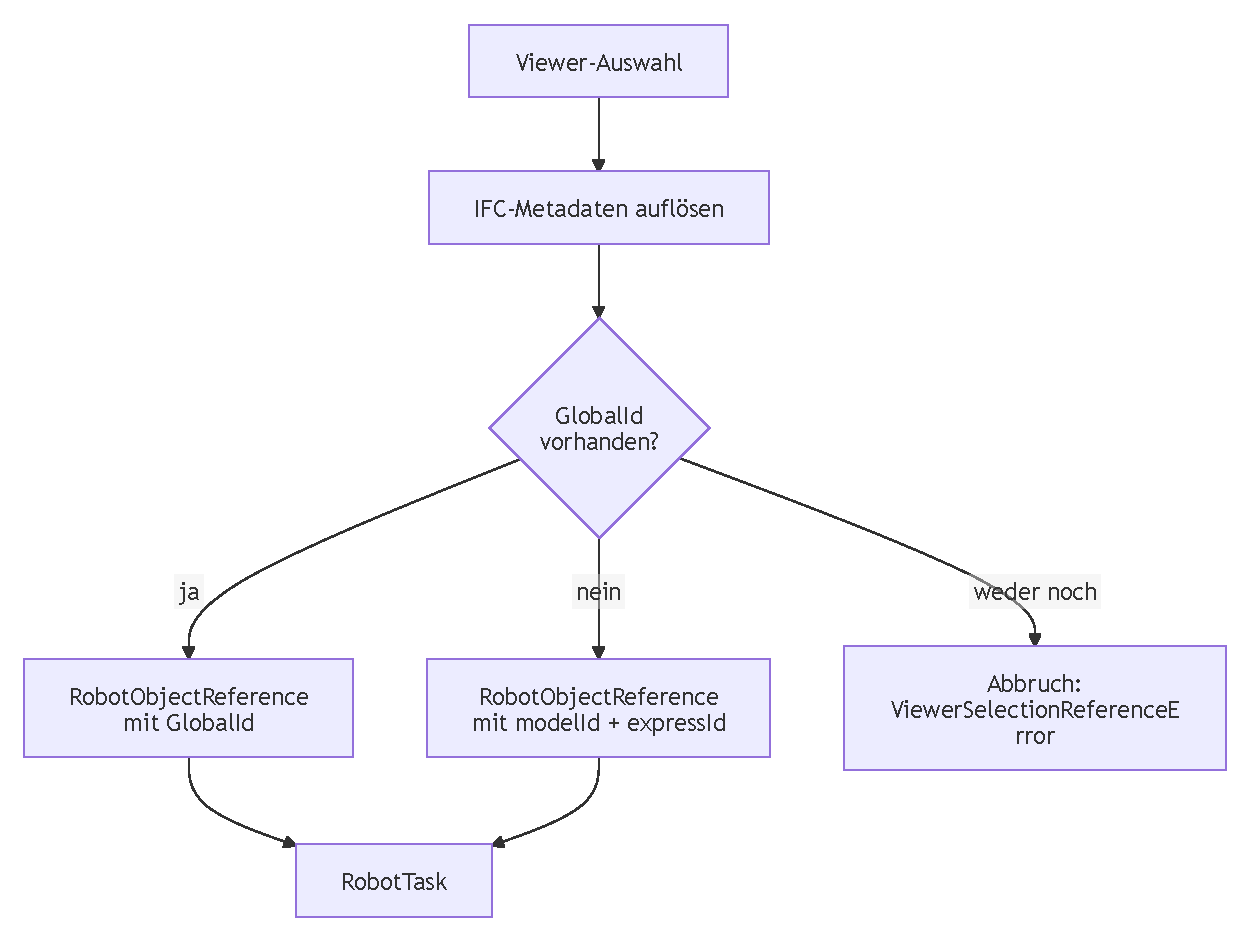
\includegraphics[width=0.4\textwidth]{pics/viewer_Objektreferenz.pdf}
    \caption{Überführung einer bestätigten Viewer-Auswahl in eine dauerhafte fachliche Objektreferenz.}
    \label{fig:viewer-Objektreferenz}
\end{figure}

\subsection{Missionshierarchie und Task-Sequenzen}\label{subsec:Hierarchie_sequenzen}
Eine Robotermission besteht aus mehreren ausführbaren Einzelschritten. Für deren Beschreibung sind
zwei Fragen zu beantworten, die auf den ersten Blick zusammenfallen, semantisch jedoch verschieden
sind: Welche Schritte gehören zu einer Mission, und in welcher Abhängigkeit stehen diese Schritte
zueinander? Das in dieser Arbeit entworfene Domänenmodell beantwortet beide Fragen getrennt.
\textit{RobotMission.tasks} bestimmt die Zugehörigkeit der Schritte zur Mission sowie deren
deterministische Darstellungsordnung, \textit{RobotMission.sequences} beschreibt die
Ausführungsabhängigkeiten zwischen diesen Schritten.

\subsubsection{Missionshierarchie}
\textit{RobotMission} bildet die übergeordnete Einheit einer zusammengehörigen Folge von
Roboteraktivitäten und fasst mehrere \textit{RobotTask}-Objekte als ausführbare Kindelemente
zusammen (vgl. Abschnitt~\ref{subsec:Internes_Domänenmodell}). Jeder Task besitzt eine stabile, anwendungsseitig vergebene Kennung.
Diese Kennung muss innerhalb einer Mission eindeutig sein, da sie als Bezugspunkt aller weiteren
Beziehungen dient: Das Hinzufügen eines Tasks wird bei bereits vergebener Kennung mit einem
Domänenfehler abgewiesen, und die Missionsvalidierung meldet doppelte Task-IDs als blockierenden
Fehler. Die Eindeutigkeit ist damit keine Konvention, sondern eine geprüfte Invariante des Modells.

Das Feld \textit{tasks} repräsentiert ausschließlich die enthaltenen Schritte. Es trägt zwar eine
Reihenfolge, weil es als Liste realisiert ist, doch diese Reihenfolge besitzt keine eigenständige
Ausführungssemantik. Sie dient der reproduzierbaren Darstellung und als stabiles Ordnungskriterium
dort, wo die Abhängigkeitsbeziehungen keine eindeutige Aussage treffen.


\subsubsection{Task-Sequenzen}
Eine \textit{RobotTaskSequence} beschreibt eine gerichtete Beziehung zwischen genau zwei Tasks. Sie
besitzt eine eigene Kennung \textit{id}, verweist über \textit{predecessorTaskId} auf den Vorgänger
und über \textit{successorTaskId} auf den Nachfolger und trägt mit \textit{sequenceType} die Art der
zeitlichen Abhängigkeit. Der Vorgänger ist derjenige Task, dessen Zustand die Ausführbarkeit des
Nachfolgers einschränkt. Der Nachfolger ist der eingeschränkte Task.

Entscheidend ist, dass eine Sequenz keine Zugehörigkeitsaussage trifft. Sie erklärt einen Task nicht
zum Bestandteil einer Mission, sondern setzt zwei bereits zur Mission gehörende Tasks zueinander in
Beziehung. Beide Endpunkte müssen deshalb auf Tasks verweisen, die in \textit{tasks} enthalten sind.
Umgekehrt kann ein Task ohne jede Sequenzbeziehung existieren. Er ist dann Bestandteil der Mission,
aber zeitlich ungebunden. Genau diese Asymmetrie zeigt, dass sich beide Informationen nicht durch
die Position eines Tasks in einem einzigen Array ausdrücken lassen: Eine Arrayposition kann weder
ausdrücken, dass zwei Schritte unabhängig voneinander ausführbar sind, noch welche Art der
zeitlichen Kopplung zwischen zwei gekoppelten Schritten gilt.

\subsubsection{Sequenztypen}
Das Modell unterstützt die Beziehungsarten \textit{FINISH\_START}, \textit{START\_START},
\textit{FINISH\_FINISH} und \textit{START\_FINISH}. Sie beschreiben, welche Zustandsübergänge des
Vorgängers den Beginn oder das Ende des Nachfolgers freigeben. Im Zentrum des betrachteten
Anwendungsfalls steht \textit{FINISH\_START}: Der Nachfolger darf erst beginnen, nachdem der Vorgänger
abgeschlossen wurde. Diese Beziehung ist der Standardwert bei der Erzeugung einer Sequenz und deckt
den typischen Fall einer linearen Missionsausführung ab.
Die übrigen drei Typen sind im Datenmodell vorhanden und werden bei der Anzeige unverändert
übernommen. Sie belegen, dass das Domänenmodell grundsätzlich auch überlappende oder endebezogene
Kopplungen ausdrücken kann. Eine gesonderte Auswertung dieser Semantik findet im gegenwärtigen Stand
jedoch nicht statt.

\subsubsection{Lineare Reihenfolge und allgemeiner Abhängigkeitsgraph}
Eine einfache Bedienoberfläche kann eine Mission als lineare Folge darstellen. Für eine solche
lineare Bearbeitung lässt sich der Missionsplan als vollständige Kette von
\textit{FINISH\_START}-Beziehungen ausdrücken, während die Hierarchieordnung als deterministische
Darstellungsordnung erhalten bleibt. Die konkrete Interaktion zum Umsortieren und Ersetzen dieser
Beziehungen wird in Kapitel~\ref{sec:Editor} behandelt.

Das zugrunde liegende Modell ist jedoch allgemeiner. Sequenzen werden als gerichteter Graph geführt
und einzeln hinzugefügt. Die Prüfung beschränkt sich auf Endpunktexistenz, Selbstbezug und
Zyklenfreiheit. Verzweigte Strukturen, also ein Vorgänger mit mehreren Nachfolgern oder ein Nachfolger
mit mehreren Vorgängern, sind daher auf Domänenebene zulässig und werden bei der Ermittlung der
Ausführungsreihenfolge auch berücksichtigt: Die Reihenfolge wird topologisch bestimmt, wobei die
Hierarchieordnung aus \textit{tasks} als stabiles Kriterium zwischen unabhängigen Zweigen dient.
Damit wird die Arbeitsteilung zwischen beiden Feldern unmittelbar sichtbar. Die Bearbeitung solcher
verzweigter Missionsgraphen wird von der aktuellen Oberfläche allerdings nicht angeboten. Dort steht
ausschließlich die lineare Umsortierung zur Verfügung.
\begin{figure}[htbp]
    \centering
    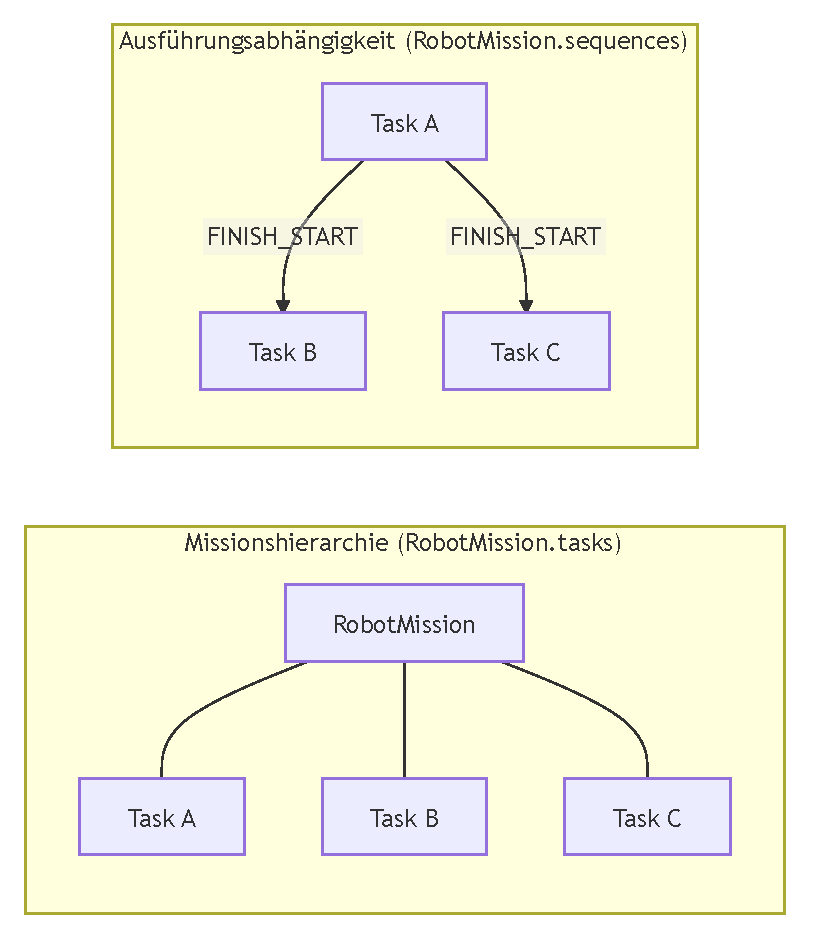
\includegraphics[width=0.4\textwidth]{pics/zugehoerigkeit_abhaengigkeit.pdf}
    \caption{Trennung von Zugehörigkeit und Abhängigkeit. Oben bestimmt \textit{tasks}, welche
Schritte zur Mission gehören. Unten beschreibt \textit{sequences}, welche Abhängigkeiten zwischen
denselben Schritten gelten.}
    \label{fig:zugehoerigkeit-abhaengigkeit}
\end{figure}


\subsubsection{Strukturelle Konsistenz der Sequenzen}
Da Sequenzen ausschließlich über Task-Kennungen definiert sind, ist ihre Gültigkeit an die
Hierarchie gebunden und maschinell prüfbar. Geprüft werden das Vorhandensein einer nicht leeren
Sequenz-ID, der Ausschluss von Selbstbezügen, die Auflösbarkeit beider Endpunkte auf bestehende
Tasks sowie die Zyklenfreiheit des gesamten Graphen. Beim Hinzufügen einer Sequenz wird zusätzlich
die Eindeutigkeit der Sequenz-ID sichergestellt. Die Bedeutung der Zyklenfreiheit lässt sich
unmittelbar einsehen: Eine Konstellation A - B - C - A
fordert von jedem beteiligten Task, vor sich selbst ausgeführt zu werden, und lässt daher keine
widerspruchsfreie Ausführungsreihenfolge zu. Sie wird deshalb als Fehler zurückgewiesen. Die
Einordnung dieser Prüfungen in die Gesamtarchitektur der Validierung erfolgt in
Abschnitt~\ref{subsec:validierungsmodell}.


\subsubsection{Bedeutung für die IFC-Abbildung}
Die getrennte Führung beider Informationen im internen Modell wird durch die IFC-Abbildung
unterstützt: IFC unterscheidet beide Aussagen durch verschiedene Beziehungsobjekte
\parencite{buildingsmart2024ifc43}. Die
Missionshierarchie wird konzeptionell auf \textit{IfcRelNests} abgebildet,
die Abhängigkeit zwischen zwei Tasks auf \textit{IfcRelSequence}. Ein Domänenmodell, das
Zugehörigkeit und Reihenfolge in einer einzigen geordneten Liste vermischte, müsste diese
Unterscheidung beim Export erst rekonstruieren und beim Import erneut auflösen. Die vollständige
Abbildung einschließlich der Attribute beider Relationen wird in
Abschnitt~\ref{subsec:modell_ifc} behandelt.

Die Verwendung von \textit{IfcRelSequence} für robotische Taskfolgen ist dabei kein neu eingeführter
Mechanismus dieser Arbeit; \textcite{slepicka2026fim} setzen die Relation bereits zur expliziten
Sequenzierung von Platzierungsaufgaben ein. Untersuchungsrelevant ist hier die getrennte und inverse
Abbildung zweier Sachverhalte: \textit{IfcRelNests} muss die Missionszugehörigkeit rekonstruierbar
halten, während \textit{IfcRelSequence} unabhängig davon die Ausführungsabhängigkeit erhält.


\subsection{Repräsentation ergänzender Taskinformationen in IFC}\label{subsec:Taskinformationen}
Mit der in Abschnitt~\ref{subsec:Hierarchie_sequenzen} beschriebenen Hierarchie aus übergeordnetem Missions-Task, ausführbaren
Teilaufgaben und deren Abhängigkeitsbeziehungen ist das Grundgerüst der Annotation festgelegt. Ein
\textit{RobotTask} trägt jedoch über diese strukturelle Einordnung hinaus Informationen, die für
eine spätere robotische Auswertung wesentlich sind: Er verweist auf konkrete Elemente des
Gebäudemodells, er beschreibt eine auszuführende Aktion mitsamt ihrer Vorbedingungen und
Erfolgskriterien, und er kann geplante sowie tatsächliche Ausführungszeiten führen. Diese drei
Informationsarten sind fachlich verschieden. Ein Objektbezug stellt eine Beziehung zwischen zwei
bereits existierenden Entitäten her, eine Aktionsangabe beschreibt projektspezifische
Robotiksemantik ohne Entsprechung im IFC-Kernschema, und eine Zeitangabe entspricht einem in IFC
bereits standardisierten Konzept. Das Annotationsmodell nutzt deshalb bewusst drei unterschiedliche
IFC-Mechanismen, statt sämtliche Zusatzinformationen einheitlich in ein benutzerdefiniertes Property
Set zu schreiben. Der vorliegende Abschnitt begründet diese Zuordnung. Die vollständige,
systematische Abbildung des Domänenmodells folgt in Abschnitt~\ref{subsec:modell_ifc}.

\subsubsection{Objektbezüge als Relationen}
Das Domänenmodell unterscheidet vier Felder, über die ein \textit{RobotTask} auf Gebäudeelemente
verweist. \textit{targetObjects} bezeichnet die unmittelbar bearbeiteten oder als Handlungskontext
genutzten Objekte, \textit{affectedObjects} die lediglich mittelbar betroffenen Objekte. Für
Bewegungsaufgaben treten \textit{startReference} als Ausgangspunkt und \textit{targetReference} als
Ziel hinzu. Diese Felder sind keine redundanten Varianten derselben Zuordnung, sondern kodieren
unterschiedliche Rollen, die dasselbe Bauteil im Kontext verschiedener Aufgaben einnehmen kann: Eine
Tür ist beim Öffnen direktes Ziel, bei einer Durchfahrt Durchgangselement und bei einer
Bewegungsaufgabe möglicherweise nur Zwischenraumgrenze. Die Domänenvalidierung behandelt diese
Rollen entsprechend differenziert, indem sie beispielsweise für \textit{OPEN}, \textit{CLOSE},
\textit{SWITCH\_ON} und \textit{SWITCH\_OFF} mindestens ein Zielobjekt und für \textit{MOVE} sowohl
Start- als auch Zielreferenz verlangt.

Die Abbildung dieser Rollen erfolgt ausschließlich relational. Beim Mapping wird aus einer
\textit{RobotObjectReference} eine externe Objektreferenz erzeugt, die neben \textit{GlobalId} und
dem modelllokalen Rückfallpaar aus Modell- und Express-ID lediglich IFC-Klasse und Namen übernimmt.
Es werden weder Geometrie noch Eigenschaften des Bauteils dupliziert, und es wird umgekehrt keine
Aktionssemantik an das Gebäudeelement geschrieben. Das annotierte Modell bleibt dadurch in seinem
bautechnischen Bestand unverändert. Die Mission wird ihm als zusätzlicher Beziehungsgraph
beigestellt.

Als Trägerbeziehung dient überwiegend \textit{IfcRelAssignsToProcess}, die einen Prozess mit den von
ihm in Anspruch genommenen Objekten verknüpft. Die konkrete Rolle wird über das
\textit{Name}-Attribut der Beziehung geführt und nimmt die Werte \textit{OPERATES\_ON},
\textit{AFFECTS}, \textit{PASSES\_THROUGH}, \textit{NAVIGATES\_TO} und \textit{MOVE\_FROM} an.
Direkte Zielobjekte erhalten dabei einen aktionsabhängigen Namen: Für \textit{PASS\_THROUGH} und
\textit{NAVIGATE\_TO} werden die spezifischeren Rollen gewählt, in allen übrigen Fällen
\textit{OPERATES\_ON}. Eine Ausnahme bildet das Bewegungsziel. Da es kein vom Prozess genutztes,
sondern ein den Prozess bestimmendes Produkt darstellt, wird es über \textit{IfcRelAssignsToProduct}
mit dem Namen \textit{MOVE\_TO} abgebildet, wobei das Zielobjekt als \textit{RelatingProduct} und
der Task als zugeordnetes Objekt auftritt. Die Richtungsumkehr gegenüber den übrigen Zuordnungen ist
damit nicht willkürlich, sondern folgt der Semantik der jeweiligen IFC-Beziehung. Weil sämtliche
Rollen als eigenständige Beziehungsobjekte mit sprechendem Namen vorliegen, lässt sich der
Objektbezug beim Reimport eindeutig in dasselbe Domänenfeld zurückführen.

\subsubsection{Projektspezifische Semantik in eigenen Property Sets}
Wo IFC bereits eine passende Semantik bereitstellt, nutzt das Annotationsmodell native Attribute:
Die Domänen-ID eines Tasks wird nach \textit{Identification} geschrieben, der Lebenszyklusstatus
nach \textit{Status}, die vierstufige Priorität in das ganzzahlige \textit{Priority}-Attribut, und
die Unterscheidung zwischen Missions- und Taskebene erfolgt über \textit{ObjectType} in Verbindung
mit einem benutzerdefinierten vordefinierten Typ. Für die eigentliche Robotiksemantik existiert eine
solche Entsprechung jedoch nicht. Weder die unterstützten Aktionsarten noch Angaben zu geforderten
Roboterfähigkeiten oder zu Vor- und Nachbedingungen lassen sich verlustfrei auf Attribute des
IFC-Kernschemas abbilden. Diese Informationen werden deshalb ergänzend über eigene Property Sets
geführt, die dem generierten \textit{IfcTask} über \textit{IfcRelDefinesByProperties} zugeordnet
werden — und ausdrücklich nur diesem, nicht den referenzierten Bauteilen.

Implementiert sind drei Property Sets. \textit{RobotAction} trägt am ausführbaren Task die
Aktionssemantik: \textit{ActionType} ist stets vorhanden, da es das angeforderte Verhalten benennt.
Optional treten \textit{TargetState}, \textit{TargetObjectRole}, \textit{AffectedObjectRole},
\textit{RequiredCapability} und \textit{SuccessCondition} als Einzelwerte sowie
\textit{Preconditions} und \textit{Postconditions} als Listenwerte hinzu. \textit{RobotTask} führt
taskbezogene Metadaten, namentlich die Änderungszeitstempel sowie die optionalen
Viewer-Annotationsdaten aus Kamerastellung und Markerposition. \textit{RobotMission} führt am
übergeordneten Missions-Task die entsprechenden Zeitstempel sowie zwei für Kompatibilität und
Wiedereinlesen wesentliche Angaben: die Version des Annotationsschemas, derzeit \textit{1.0.0}, und
ein boolesches Kennzeichen, ob die Mission einen fachlich gesetzten Zeitplan besitzt. Der
reservierte Präfix \textit{Pset\_} wird für diese Sets nicht verwendet. Der Writer bricht den Export
ab, sobald ein Property-Set-Name mit diesem Präfix beginnt. Die zugrunde liegende Designentscheidung
lässt sich damit knapp fassen: Standardisierte IFC-Strukturen werden genutzt, wo eine passende
Semantik vorhanden ist, während projektspezifische Robotiksemantik ergänzend und klar erkennbar
abgegrenzt in eigenen Property Sets abgelegt wird.

\subsubsection{Zeitinformationen über native IFC-Strukturen}
Zeitangaben bilden den Gegenfall zur Aktionssemantik. Die Domänenstruktur \textit{RobotTaskTime}
führt geplanten Start, geplantes Ende, geplante Dauer, tatsächliche Start- und Endzeitpunkte, die
verbleibende Restdauer sowie einen Fertigstellungsgrad. Für solche Angaben stellt IFC mit
\textit{IfcTaskTime} eine native Struktur bereit. Deren Verwendung für taskbezogene Bauabläufe ist
unter anderem bei \textcite{sheik2023exchanging} und für einen robotischen Prozess bei
\textcite{slepicka2026fim} belegt. Das Annotationsmodell übernimmt diesen etablierten Mechanismus als
einen Bestandteil der rekonstruierbaren Missionsannotation. Zeitinformationen werden daher nicht
als beliebige Custom Properties, sondern über das native \textit{TaskTime}-Attribut des zugehörigen
\textit{IfcTask} abgebildet. Die Werte werden entsprechend den typisierten IFC-Wertarten
repräsentiert; der Fertigstellungsgrad wird beispielsweise als positives Verhältnis geführt.

Der für diese Arbeit spezifische Gesichtspunkt liegt nicht in der Einführung von \textit{IfcTaskTime}, sondern
darin, dass die Zeitinformation beim Import wieder demselben identifizierbaren Task zugeordnet und
gemeinsam mit dessen Aktionssemantik, Objektbezügen, Objektrollen, Abhängigkeiten und Missionskontext
rekonstruiert werden kann. Dies betrifft die persistente zeitliche Repräsentation. Ob geplante
Zeiträume, Dauern oder zeitliche Zielvorgaben bei der Ausführung eingehalten werden können, muss eine
nachgelagerte Scheduling- oder Ausführungskomponente beurteilen. Das IFC-Schema erzwingt weder die
Konsistenz der eingetragenen Zeitwerte noch die Einhaltung von Deadlines
\parencite{buildingsmart2024ifc43}.

Auf Missionsebene wird die optionale Struktur \textit{RobotMissionSchedule} auf
\textit{IfcWorkSchedule} abgebildet und über \textit{IfcRelAssignsToControl} mit dem übergeordneten
Missions-Task verbunden. Bemerkenswert ist, dass ein Zeitplan auch dann deterministisch erzeugt
wird, wenn die Mission keinen fachlich gesetzten Plan besitzt. Die Unterscheidung zwischen technisch
notwendiger Infrastruktur und fachlicher Planungsaussage bleibt jedoch erhalten, weil sie über die
genannte Kennzeichnung im Property Set \textit{RobotMission} explizit festgehalten wird. Damit
entsteht kein Informationsverlust, obwohl der IFC-Graph in beiden Fällen strukturell gleich
aufgebaut ist.
\subsubsection{Zusammenführung}
Die drei Bereiche folgen damit einem gemeinsamen Auswahlprinzip: Nicht die Herkunft der Information
aus dem Missionsmodell, sondern ihre Bedeutung bestimmt den IFC-Mechanismus. Beziehungen zwischen
bestehenden Entitäten werden als Beziehungsobjekte modelliert, standardisierbare Sachverhalte über
native Entitäten und Attribute, und ausschließlich die anwendungsspezifische Semantik wird über
projektspezifische Strukturen ergänzt. Der Umfang der eigenen Property Sets bleibt dadurch begrenzt und beschreibt
genau jene Semantik, für die IFC keine Entsprechung anbietet.
\begin{figure}[htbp]
    \centering
    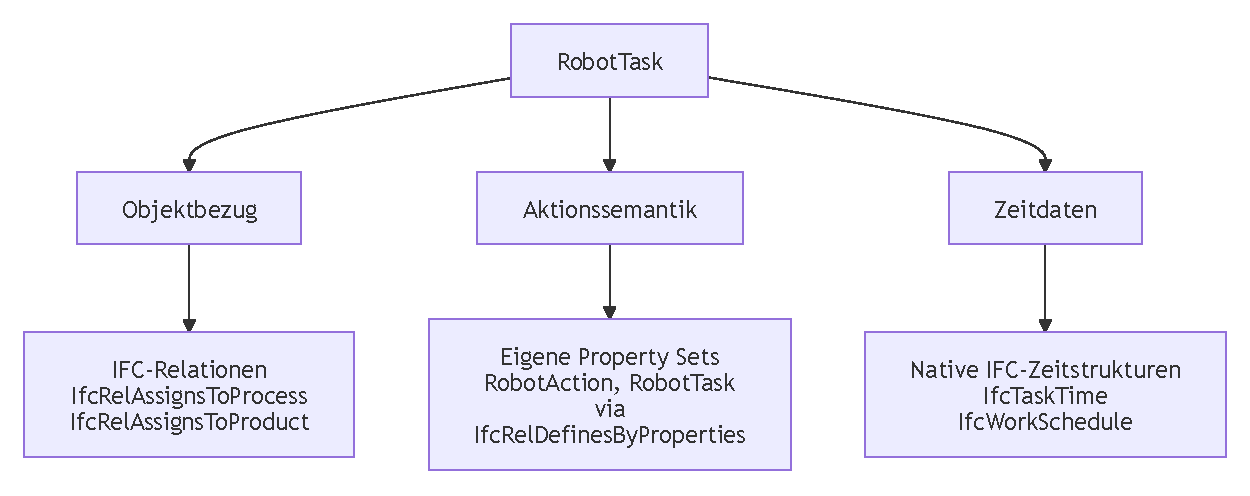
\includegraphics[width=0.6\textwidth]{pics/Informationsarten_RobotTask.pdf}
    \caption{Zuordnung der drei Informationsarten eines \textit{RobotTask} zu den jeweils verwendeten IFC-Repräsentationsmechanismen.}
    \label{fig:Informationsarten-RobotTask}
\end{figure}

Aus dieser Aufteilung ergibt sich zugleich die Aufgabe des folgenden Abschnitts. Die hier einzeln
begründeten Mechanismen greifen im erzeugten Modell ineinander: Derselbe \textit{IfcTask} ist
Ausgangspunkt mehrerer Zuweisungsbeziehungen, Träger zweier Property Sets und Inhaber eines
Zeitobjekts, während er zugleich in Hierarchie- und Abfolgebeziehungen eingebettet ist.
Abschnitt~\ref{subsec:modell_ifc} führt diese Einzelmechanismen deshalb zu einer geschlossenen
Darstellung zusammen und zeigt
systematisch, wie das vollständige interne Domänenmodell aus \textit{RobotMission} und
\textit{RobotTask} auf den resultierenden IFC-Graphen abgebildet wird.


\subsection{Abbildung des Domänenmodells auf IFC}\label{subsec:modell_ifc}

\subsubsection{Grundprinzip der Abbildung}
Die in den Abschnitten~\ref{subsec:Internes_Domänenmodell} bis
\ref{subsec:Taskinformationen} einzeln eingeführten Modellierungsentscheidungen werden hier zu
einer geschlossenen Abbildungsvorschrift zusammengeführt. Leitfrage ist, wie die
\textit{RobotMission} mit ihren \textit{RobotTask}-Objekten, deren Beziehungen und deren
Zusatzinformationen systematisch auf IFC-Entitäten und IFC-Relationen abgebildet und aus diesen
wieder rekonstruiert werden kann. Die einzelnen IFC-Entitäten werden dabei als etablierte
Mechanismen eingesetzt. Gegenstand der Designentscheidung ist ihre konkrete Kombination für das
Domänenmodell dieser Arbeit und die Eindeutigkeit der inversen Abbildung.

Die Abbildung erfolgt über drei getrennte Ebenen: das interne Domänenmodell, eine IFC-nahe
Mappingrepräsentation und die konkreten IFC-Entitäten und -Relationen. Das Domänenmodell bleibt frei
von STEP-Syntax und serialisierungslokalen Kennungen. Die mittlere Ebene beschreibt den zu
erzeugenden Relationsgraphen, ohne bereits eine Datei zu verändern; erst die äußere Ebene übernimmt
die konkrete IFC-Serialisierung. Dadurch sind die fachlichen Mappingregeln unabhängig von der
Serialisierungstechnik prüfbar, und die Domäne bleibt frei von Infrastrukturabhängigkeiten. Eine
Mission wird nur abgebildet, wenn ihre Validierung keine blockierenden Fehler meldet. Die technische
Exportpipeline wird in Kapitel~\ref{sec:Editor} behandelt.

\subsubsection{Mission und Tasks}
Sowohl die Mission als auch die ausführbaren Einzelschritte werden auf \textit{IfcTask} abgebildet.
Diese Entscheidung nutzt aus, dass \textit{IfcTask} in IFC nicht auf elementare Arbeitsschritte
beschränkt ist, sondern auch als zusammenfassender Prozessknoten verwendet werden kann.
\textit{RobotMission} bedeutet hierbei ein übergeordneter IfcTask, \textit{RobotTask} ein untergeordneter.

Beide Rollen werden im Recordgraphen explizit unterschieden (\textit{role: \dq{}MISSION\dq{} |
\dq{}EXECUTABLE\_TASK\dq{}}) und in IFC über \textit{ObjectType} markiert: Der Missionsknoten trägt
\textit{RobotMission}, die ausführbaren Schritte tragen \textit{RobotTask}. Die stabile
Domänenkennung wird jeweils in \textit{Identification} geschrieben, sodass die Zuordnung zwischen
Domänenobjekt und IFC-Entität nicht von einer Express-ID abhängt. \textit{PredefinedType} wird beim
Schreiben durchgängig auf \textit{USERDEFINED} gesetzt, weil die Robotiksemantik durch das
Aufzählungsspektrum von \textit{IfcTaskTypeEnum} nicht abgedeckt ist. Optionale Domänenangaben
werden auf vorhandene Attribute abgebildet: \textit{status} auf \textit{Status}, \textit{priority}
auf die IFC-Ganzzahlskala von 1 (niedrig) bis 4 (kritisch).

Die Mission bildet damit den übergeordneten fachlichen Kontext, ohne selbst ausführbar zu sein. Die Robotiksemantik im engeren Sinne liegt ausschließlich an den untergeordneten Tasks.

\subsubsection{Hierarchie und Sequenzen}

Die in Abschnitt~\ref{subsec:Hierarchie_sequenzen} begründete Trennung von Enthaltensein und
Ausführungsabhängigkeit wird auf IFC-Ebene durch zwei verschiedene Relationstypen abgebildet.

Erstens, pro Mission wird genau eine \textit{IfcRelNests}-Relation erzeugt, deren
\textit{RelatingObject} der Missionsknoten ist und deren \textit{RelatedObjects} die untergeordneten
Tasks in der Reihenfolge der Missionsliste enthalten.
Zweitens, für jede Domänensequenz wird dagegen eine eigene \textit{IfcRelSequence}-Relation mit
Vorgänger- und Nachfolgerprozess sowie dem übernommenen Sequenztyp erzeugt. Die stabile Sequenz-ID
der Domäne wird in \textit{Name} abgelegt.

Entscheidend ist, dass beide Strukturen unabhängig voneinander sind: Die Nesting-Reihenfolge ist
eine Darstellungs- und Zugehörigkeitsordnung, keine Ausführungsreihenfolge. Eine Mission ohne
Sequenzen bleibt hierarchisch vollständig, besitzt aber keine zeitlichen Abhängigkeiten.

\subsubsection{Objektbezüge}

Die zuvor eingeführten Rollen von Objektzuordnungen werden auf zwei IFC-Zuweisungsrelationen
abgebildet. Maßgeblich ist dabei, in welcher Rolle ein Gebäudeobjekt am Task beteiligt ist:

- Direkt adressierte Zielobjekte werden über \textit{IfcRelAssignsToProcess} an den Task gebunden.
Der Relationsname wird aus dem Aktionstyp abgeleitet: \textit{PASS\_THROUGH} ergibt
\textit{PASSES\_THROUGH}, \textit{NAVIGATE\_TO} ergibt \textit{NAVIGATES\_TO}, alle übrigen Aktionen
ergeben \textit{OPERATES\_ON}.
- Indirekt betroffene Objekte werden über eine zweite \textit{IfcRelAssignsToProcess}-Relation mit dem Namen \textit{AFFECTS} abgebildet.
- Bei \textit{MOVE}-Aufgaben wird die Startreferenz als \textit{IfcRelAssignsToProcess} mit dem
Namen \textit{MOVE\_FROM} abgebildet, die Zielreferenz dagegen als \textit{IfcRelAssignsToProduct}
mit dem Namen \textit{MOVE\_TO}.

Die unterschiedliche Behandlung von Start und Ziel folgt der IFC-Richtungslogik: Bei
\textit{IfcRelAssignsToProcess} ist der Task der zuweisende Prozess und das Gebäudeobjekt das
zugewiesene Objekt. Bei \textit{IfcRelAssignsToProduct} ist das Produkt der Bezugspunkt, dem der
Task zugeordnet wird. Das Bewegungsziel wird damit als produktbezogener Zielpunkt und nicht als vom
Task verarbeitetes Objekt modelliert. Referenzierte Gebäudeobjekte werden im Recordgraphen
ausdrücklich als modellexterne Referenzen geführt und nicht als erzeugte Entitäten. Die zugrunde
liegende Identifikationsstrategie wurde in Abschnitt~\ref{subsec:Referenzierung_IFC-Objekten} behandelt.

\subsubsection{Aktions- und Metadaten}

Prozessstruktur und Beziehungen lassen sich vollständig mit regulären IFC-Entitäten ausdrücken. Die
projektspezifische Robotiksemantik besitzt dagegen keine normative IFC-Entsprechung und wird deshalb
über drei eigene Property Sets ergänzt, die über \textit{IfcRelDefinesByProperties} an den
jeweiligen \textit{IfcTask} gebunden werden:

- \textit{RobotAction} am ausführbaren Task trägt den Aktionstyp sowie die optionalen Aktionsparameter. Mehrwertige Angaben wie Vor- und Nachbedingungen werden als Listenwerte abgelegt.
- \textit{RobotTask} am ausführbaren Task trägt Zeitstempel der Bearbeitung sowie optionale Viewer-Annotationen.
- \textit{RobotMission} am Missionsknoten trägt Missionszeitstempel, die Version des Annotationsschemas und einen Marker für einen explizit gepflegten Missionsplan.

Die Namen der Property Sets verwenden bewusst nicht den reservierten Präfix \textit{Pset\_}. Der
Export bricht ab, wenn ein solcher Name auftreten würde. Damit gilt als zentrale Regel:
\textbf{Die regulären IFC-Entitäten bilden Prozessstruktur und Beziehungen ab. Projektspezifische
Robotiksemantik wird ergänzend über eigene Property Sets gespeichert.}

\subsubsection{Zeitinformationen und Missionsplan}

Zeitliche Angaben werden nicht über eigene Property Sets, sondern über die dafür vorgesehenen
IFC-Strukturen abgebildet. \textit{RobotTaskTime} wird auf \textit{IfcTaskTime} abgebildet und
direkt als Attribut des zugehörigen \textit{IfcTask} referenziert. Die Relation entsteht also nicht
über eine Eigenschaftszuweisung. Der Missionsplan wird auf \textit{IfcWorkSchedule} abgebildet und
über \textit{IfcRelAssignsToControl} mit dem Missionsknoten verbunden.

Diese Infrastruktur wird für jede Mission erzeugt, auch wenn das Domänenmodell keinen expliziten
\textit{RobotMissionSchedule} besitzt. In diesem Fall werden Kennung, Name und Startzeit
deterministisch aus der Mission abgeleitet. Die Unterscheidung zwischen fachlich gepflegtem und
technisch erzeugtem Plan bleibt dennoch erhalten, weil sie im \textit{RobotMission}-Property-Set
explizit markiert wird.

\subsubsection{Gesamtübersicht des Mappings}

\begin{table}[htbp]
  \centering
  \small
  \renewcommand{\arraystretch}{1.3}
  \begin{tabularx}{\textwidth}{@{}|>{\raggedright\arraybackslash}p{0.33\textwidth}|X|@{}}
    \hline
    \textbf{Domänenkonzept} & \textbf{IFC-Abbildung} \\
    \hline
    \texttt{RobotMission}
      & übergeordneter \texttt{IfcTask}, \texttt{ObjectType = RobotMission} \\
    \hline
    \texttt{RobotTask}
      & untergeordneter \texttt{IfcTask}, \texttt{ObjectType = RobotTask} \\
    \hline
    Missionshierarchie
      & \texttt{IfcRelNests} \\
    \hline
    Task-Abhängigkeit (\texttt{RobotTaskSequence})
      & \texttt{IfcRelSequence}, Domänen-ID in \texttt{Name} \\
    \hline
    direkt adressierte Zielobjekte
      & \texttt{IfcRelAssignsToProcess} mit \texttt{OPERATES\_ON}, \texttt{PASSES\_THROUGH} oder \texttt{NAVIGATES\_TO} \\
    \hline
    betroffene Objekte
      & \texttt{IfcRelAssignsToProcess} mit \texttt{AFFECTS} \\
    \hline
    \texttt{MOVE}-Startreferenz
      & \texttt{IfcRelAssignsToProcess} mit \texttt{MOVE\_FROM} \\
    \hline
    \texttt{MOVE}-Zielreferenz
      & \texttt{IfcRelAssignsToProduct} mit \texttt{MOVE\_TO} \\
    \hline
    \texttt{RobotTaskTime}
      & \texttt{IfcTaskTime} als direktes \texttt{IfcTask}-Attribut \\
    \hline
    \texttt{RobotMissionSchedule}
      & \texttt{IfcWorkSchedule} mit \texttt{IfcRelAssignsToControl} \\
    \hline
    Aktionssemantik
      & Property Set \texttt{RobotAction} \\
    \hline
    Task-Metadaten
      & Property Set \texttt{RobotTask} \\
    \hline
    Missionsmetadaten und Schemaversion
      & Property Set \texttt{RobotMission} \\
    \hline
  \end{tabularx}
  \caption{Systematische Abbildung des internen Robotermissionsmodells auf IFC-Strukturen}
  \label{tab:mapping-domaene-ifc}
\end{table}
\FloatBarrier

\subsubsection{Anforderung an die bidirektionale Abbildung}
Für den Missionsroundtrip genügt es nicht, lediglich eine Serialisierungsvorschrift vom
Domänenmodell nach IFC zu definieren. Die erzeugte IFC-Struktur muss zusätzlich so eindeutig
interpretierbar sein, dass aus dem IFC-Missionsgraphen wieder eine fachlich vergleichbare
\textit{RobotMission} entsteht.

Dazu muss die inverse Abbildung mindestens die Identität der Mission und ihrer Tasks, die
Aktionssemantik, sämtliche Gebäudereferenzen und deren Rollen, die Missionszugehörigkeit, die
Ausführungsabhängigkeiten, die Task-Zeitinformationen sowie einen fachlich gesetzten Missionsplan
rekonstruieren können. Jede Missionsentität muss außerdem anhand stabiler Marker als projekteigen
erkennbar und von fremden IFC-Inhalten unterscheidbar sein. Das leisten die
\textit{ObjectType}-Werte, der \textit{USERDEFINED}-Typ und die eigenen Property-Set-Namen. Missions-,
Task- und Sequenzkennungen werden explizit in Attributen gespeichert, statt nur aus der
Graphstruktur abgeleitet zu werden. Semantisch belegte Relationsnamen erhalten die Rollen der
Objektzuordnungen, während ein gesonderter Marker technisch erzeugte Schedule-Infrastruktur von
einem fachlich gepflegten Missionsplan unterscheidet.

Die Rekonstruktion allein weist noch keinen Bedeutungserhalt nach. Das rekonstruierte Aggregat muss
mit dem beabsichtigten Domänenzustand semantisch vergleichbar sein, sodass Abweichungen bei
Identitäten, Rollen, Hierarchie, Abhängigkeiten, Zeiten oder Aktionsangaben sichtbar werden. Dieser
Anspruch ist auf die vom System verwaltete \textit{RobotMission}-Annotation begrenzt und bezeichnet
keinen allgemeinen verlustfreien IFC-Roundtrip. Die technische Umsetzung von Import,
Replacement-Export, Roundtrip-Koordination, semantischem Vergleich und Quellverwaltung wird in
Kapitel~\ref{sec:Editor} beschrieben.

\subsubsection{Version des Annotationsschemas}

Das Mapping schreibt in das \textit{RobotMission}-Property-Set eine eigene Versionsangabe des
Annotationsmodells, die als Konstante zentral gepflegt wird und aktuell den Wert \textit{1.0.0}
besitzt. Sie erlaubt es, projekteigene Missionsannotationen eindeutig als solche zu erkennen und
spätere Änderungen des eigenen Annotationsschemas kontrolliert zu behandeln. Annotationen ohne diese
Angabe werden beim Lesen als Altbestand behandelt und über definierte Kompatibilitätsregeln
interpretiert.

Diese Version ist strikt von der IFC-Schemaversion zu unterscheiden. IFC4 beziehungsweise IFC4X3
beschreiben das zugrunde liegende Datenschema, während die Annotationsversion ausschließlich die
projektspezifische Missionsmodellierung innerhalb dieses Schemas versioniert. Für das Mapping selbst
ist die IFC-Schemaversion nachrangig: Alle verwendeten Entitäten und Relationen existieren in beiden
unterstützten Schemafamilien, sodass die Schemawahl lediglich die beim Schreiben verwendeten
Konstruktoren bestimmt und die Abbildungsvorschrift unverändert lässt.

\subsection{Validierungsmodell}\label{subsec:validierungsmodell}
\subsubsection{Motivation und Fragestellung}
Ein Annotationsmodell besteht nicht ausschließlich aus Datenstrukturen. Eine Datenstruktur kann
syntaktisch korrekt befüllt sein und dennoch eine fachlich sinnlose Robotermission beschreiben: ein
Task ohne Zielobjekt, eine Bewegung ohne Startpunkt oder ein Abhängigkeitsgraph ohne
widerspruchsfreie Ausführungsreihenfolge. Dieser Abschnitt beantwortet deshalb die Frage, welche
fachlichen Invarianten eine Mission erfüllen muss, damit sie innerhalb des Modells als konsistent
gilt.

Die Validierung ist eine Verantwortung der Domäne und nicht der Benutzeroberfläche. Sie bleibt damit
unabhängig von Viewer, Persistenz und IFC-Serialisierung und gilt gleichermaßen für bearbeitete,
vor dem Export stehende und aus IFC rekonstruierte Missionen. Die Prüfung sammelt Befunde, statt beim
ersten Verstoß abzubrechen, sodass ein vollständiges Bild des Missionszustands entsteht.

\subsubsection{Strukturelle Validierung}
Die strukturelle Ebene sichert die Identität und Vollständigkeit des Aggregats. Eine
\textit{RobotMission} benötigt eine nicht leere Kennung und einen nicht leeren Namen sowie
mindestens einen ausführbaren Task. Jeder \textit{RobotTask} benötigt ebenfalls Kennung und Name.
Task-Kennungen müssen innerhalb einer Mission eindeutig sein, weil Hierarchie und Sequenzbeziehungen
ausschließlich über diese Kennungen aufgelöst werden. Der Aktionstyp wird zur Laufzeit gegen die
Menge der unterstützten Werte geprüft, da deserialisierte Daten die statische Typisierung umgehen
können. Ein fehlender und ein unbekannter Aktionswert werden dabei unterschieden.

Ein Teil dieser Invarianten wird bereits durch die Domänenoperationen konstruktiv erzwungen: Leere
Kennungen oder Namen sowie doppelte Task- und Sequenzkennungen führen unmittelbar zu einem
Domänenfehler. Die deklarative Validierung bleibt dennoch notwendig, weil Missionen auch aus
Persistenz oder IFC-Import stammen können.

\subsubsection{Aktionsbezogene Validierung}
Aktionstypen stellen unterschiedliche Anforderungen an einen Task. Direkt manipulierende Aktionen
(\textit{OPEN}, \textit{CLOSE}, \textit{SWITCH\_ON}, \textit{SWITCH\_OFF}) verlangen mindestens ein
Zielobjekt, \textit{PASS\_THROUGH} mindestens eine Objektreferenz, die wahlweise als Ziel- oder als
betroffenes Objekt hinterlegt sein darf. \textit{MOVE} verlangt sowohl eine Start- als auch eine
Zielreferenz, da eine Bewegung ohne beide Endpunkte nicht ausführbar beschrieben ist. Für
\textit{NAVIGATE\_TO} sind keine zusätzlichen Anforderungen implementiert.

Darüber hinaus wird die Aktionssemantik gegen den Objektbezug geprüft: Für türbezogene und
schalterbezogene Aktionen wird die bekannte IFC-Klasse der Zielobjekte auf Plausibilität untersucht.
Eine bekannte, aber unpassende Klasse gilt als Fehler. Eine fehlende Klasseninformation wird
lediglich als Warnung geführt, weil die Annotation trotzdem zutreffend sein kann. Schließlich stellt
die Validierung sicher, dass Aktionsparameter am Task und nicht an einer Objektreferenz hängen:
Referenzen, die aktionsspezifische Eigenschaften mitführen, werden zurückgewiesen. Damit wird die in
Abschnitt~\ref{subsec:Modellierung_Roboteraktionen} begründete Trennung von Objektidentität und Aktionssemantik auch gegen fremde oder
ältere Daten durchgesetzt.

\subsubsection{Referenzvalidierung}
Die Referenzvalidierung fragt nicht, wie eine Referenz technisch aufgelöst wird — dies wurde in
Abschnitt~\ref{subsec:Referenzierung_IFC-Objekten} behandelt —, sondern ob die gespeicherte Referenz im Kontext der Mission zulässig und
verwendbar ist. Geprüft werden alle referenztragenden Felder eines Tasks gemeinsam: Ziel- und
betroffene Objekte sowie Start- und Zielreferenz. Eine vorhandene, aber leere \textit{GlobalId} ist
unzulässig. Ein \textit{expressId}-Wert muss eine nicht negative ganze Zahl sein. Eine rein
modelllokale Referenz ohne \textit{GlobalId} erfordert zwingend eine Modellkennung, da sie
andernfalls außerhalb ihres Ursprungsmodells nicht mehr eindeutig ist.

\subsubsection{Sequenz- und Graphvalidierung}
Die Abhängigkeiten zwischen Tasks werden getrennt vom Hierarchiebaum geprüft. Jede Sequenz benötigt
eine Kennung. Vorgänger und
Nachfolger müssen auf Tasks derselben Mission verweisen, und ein Task darf nicht sein eigener
Vorgänger sein. Ergänzend wird der gesamte gerichtete Graph über eine Tiefensuche auf Zyklen
untersucht.

Ein solcher Zyklus (z.B. Task A $\rightarrow$ Task B $\rightarrow$ Task A) besitzt keine widerspruchsfreie
Ausführungsreihenfolge und wird deshalb als Fehler gemeldet. Die Ordnungsfunktion des Modells
verhält sich dazu konsistent: Lässt sich keine vollständige topologische Reihenfolge bilden, wird
die Hierarchieordnung unverändert zurückgegeben, sodass keine Tasks stillschweigend verschwinden,
während die Validierung den Widerspruch ausweist. Auch Operationen, die den Graphen verändern,
prüfen den vollständigen resultierenden Graphen und schlagen atomar fehl, statt eine zyklische
Zwischenlage zu erzeugen.

\subsubsection{Fehler und Warnungen}
Das Modell kennt genau zwei Schweregrade. Fehler kennzeichnen eine fachlich ungültige Mission und
blockieren die Weiterverarbeitung. Warnungen kennzeichnen Unsicherheit, die die Gültigkeit nicht
aufhebt. In der aktuellen Implementierung ist die fehlende IFC-Klasseninformation eines Zielobjekts
der einzige als Warnung geführte Befund — alle übrigen Regeln sind blockierend. Jeder Befund trägt
einen stabilen Code sowie optional Task- und Sequenzbezug, sodass Aufrufer nicht auf Meldungstexte
angewiesen sind.

\begin{table}[htbp]
  \centering
  \small
  \renewcommand{\arraystretch}{1.3}
  \begin{tabularx}{\textwidth}{@{}|>{\raggedright\arraybackslash}p{0.14\textwidth}|X|>{\raggedright\arraybackslash}p{0.22\textwidth}|@{}}
    \hline
    \textbf{Validierungs-ebene} & \textbf{Beispielhafte Prüfung} & \textbf{Zweck} \\
    \hline
    Struktur & nicht leere und eindeutige Task-Kennungen, Pflichtnamen, mindestens ein Task & konsistentes Domänenobjekt \\
    \hline
    Aktion & Zielobjekt bzw. Start-/Zielreferenz je Aktionstyp, plausible IFC-Klasse & fachlich sinnvoller Task \\
    \hline
    Referenz & gültige \texttt{GlobalId} bzw. \texttt{modelId} + \texttt{expressId}, keine Aktionsparameter an der Referenz & gültige Verknüpfung \\
    \hline
    Sequenz & Sequenz-Kennung, existierende Endpunkte, keine Selbstreferenz & konsistenter Missionsgraph \\
    \hline
    Graph & keine Zyklen & ausführbare Abhängigkeiten \\
    \hline
    Zeit & Fertigstellungsgrad im Bereich 0 bis 1 & konsistentes Zeitmodell \\
    \hline
  \end{tabularx}
\end{table}

\subsubsection{Validierung vor dem Export}
Eine syntaktisch erzeugbare IFC-Datei ist nicht automatisch eine fachlich gültige
Robotermissionsannotation. Das Modell prüft daher bereits vor dem Schreiben: Die Abbildung des
Domänenmodells auf IFC-nahe Records bricht ab, sobald blockierende Validierungsfehler vorliegen.
Unvollständige Tasks oder zyklische Graphen können damit gar nicht erst in eine Form gebracht
werden, die wie eine exportfertige Annotation aussieht. Die technische Exportpipeline selbst wird im
Implementierungskapitel behandelt.

\subsubsection{Validierung während des  Imports}
Die inverse Richtung nutzt dieselben Regeln. Eine aus IFC rekonstruierte Mission durchläuft die
vollständige Domänenvalidierung. Die Befunde werden als Importbefunde mit vorangestelltem
Domänen-Präfix übernommen. Enthält die Rekonstruktion Fehler, gilt die betroffene Mission als
ungültig und wird verworfen. Da jeder Missionsknoten unabhängig rekonstruiert wird, bleiben andere,
in sich gültige Missionen derselben Datei importierbar. Auf Roundtrip-Ebene wird eine IFC-Quelle,
deren eigene Annotationen fehlerhaft sind, als unsicher markiert. Ein Export in diese Quelle wird
anschließend verweigert, um bekannt fehlerhafte Annotationen nicht zu überschreiben oder
fortzuschreiben.

\subsubsection{Abgrenzung zum semantischen Roundtrip-Vergleich}
Die Domänenvalidierung prüft die interne Gültigkeit einer einzelnen Mission: Pflichtfelder,
Referenzen, Aktionsregeln, Sequenzgraph und Zeitwerte. Der semantische Vergleich prüft demgegenüber
eine Relation zwischen zwei Aggregaten, nämlich ob die nach dem Export erneut importierte Mission
dem beabsichtigten Domänenmodell entspricht. Eine rekonstruierte Mission kann intern gültig sein und
dennoch fachlich vom Ausgangszustand abweichen, etwa durch eine veränderte Objektrolle oder eine
fehlende Abhängigkeit. Beide Prüfarten sind deshalb getrennt und wirken im Roundtrip komplementär.
Der semantische Vergleich bildet damit einen wesentlichen Teil der konzeptionellen Antwort auf F3
und wird hinsichtlich seiner technischen Durchführung in Kapitel~\ref{sec:Editor} vertieft.
